%%%%%%%%%%%%%%%%%%%%%%%%%%%%%%%%%%%%%%%%%
% Masters/Doctoral Thesis 
% LaTeX Template
% Version 1.43 (17/5/14)
%
% This template has been downloaded from:
% http://www.LaTeXTemplates.com
%
% Original authors:
% Steven Gunn 
% http://users.ecs.soton.ac.uk/srg/softwaretools/document/templates/
% and
% Sunil Patel
% http://www.sunilpatel.co.uk/thesis-template/
%
% License:
%  CC BY-NC-SA 3.0 (http://creativecommons.org/licenses/by-nc-sa/3.0/)
%
% Note:
% Make sure to edit document variables in the Thesis.cls file
%
%%%%%%%%%%%%%%%%%%%%%%%%%%%%%%%%%%%%%%%%%

%----------------------------------------------------------------------------------------
%  PACKAGES AND OTHER DOCUMENT CONFIGURATIONS
%----------------------------------------------------------------------------------------

\documentclass[12pt, oneside]{Thesis} % The default font size and one-sided printing (no margin offsets)

\graphicspath{{Pictures/}} % Specifies the directory where pictures are stored

\usepackage[square, numbers, comma, sort&compress]{natbib} % Use the natbib reference package - read up on this to edit the reference style; if you want text (e.g. Smith et al., 2012) for the in-text references (instead of numbers), remove 'numbers' 
\hypersetup{urlcolor=black, colorlinks=true} % Colors hyperlinks black
\title{\ttitle} % Defines the thesis title

\usepackage{graphicx}
\usepackage{enumitem}
\usepackage{tabularx}
\usepackage{subcaption}

% Enable red text to signify todos
\usepackage{xcolor}
\newcommand\todo[1]{\textcolor{teal}{#1}} %magenta?
\newcommand\advice[1]{\textcolor{red}{#1}}
\newcommand\nice[1]{\textcolor{green}{#1}}

\begin{document}

\frontmatter % Use roman page numbering style (i, ii, iii, iv...) for the pre-content pages

\setstretch{1.3} % Line spacing of 1.3

% Define the page headers using the FancyHdr package and set up for one-sided printing
\fancyhead{} % Clears all page headers and footers
\rhead{\thepage} % Sets the right side header to show the page number
\lhead{} % Clears the left side page header

\pagestyle{fancy} % Finally, use the "fancy" page style to implement the FancyHdr headers

\newcommand{\HRule}{\rule{\linewidth}{0.5mm}} % New command to make the lines in the title page

%  PDF meta-data
\hypersetup{pdftitle={\ttitle}}
\hypersetup{pdfsubject=\subjectname}
\hypersetup{pdfauthor=\authornames}
\hypersetup{pdfkeywords=\keywordnames}

%----------------------------------------------------------------------------------------
%  TITLE PAGE
%----------------------------------------------------------------------------------------

\begin{titlepage}
\begin{center}

\textsc{\LARGE \univname}\\[1.5cm] % University name
\textsc{\Large Master of Science}\\[0.5cm] % Thesis type

\HRule \\[0.4cm] % Horizontal line
{\huge \bfseries \ttitle}\\[0.4cm] % Thesis title
\HRule \\[1.5cm] % Horizontal line
 
\begin{minipage}{0.4\textwidth}
\begin{flushleft} \large
\emph{Author:}\\
{\authornames} % Author name
\end{flushleft}
\end{minipage}
\begin{minipage}{0.4\textwidth}
\begin{flushright} \large
\emph{Supervisor:} \\
\href{\supurl}{\supname} % Supervisor name - remove the \href bracket to remove the link  
\end{flushright}
\end{minipage}\\[3cm]
 
%\groupname\
\deptname\ % Research group name and department name
 
{\large \today}\\[4cm] % Date

\includegraphics{Figures/logo-ntnu.png} % University/department logo - uncomment to place it
 
\vfill
\end{center}

\end{titlepage}

%----------------------------------------------------------------------------------------
%	ABSTRACT PAGE
%----------------------------------------------------------------------------------------

\addtotoc{Abstract} % Add the "Abstract" page entry to the Contents

\abstract{\addtocontents{toc}{\vspace{1em}} % Add a gap in the Contents, for aesthetics

\todo{This page should hold the abstract, which should be a short summary of the paper.}

\clearpage % Start a new page

%----------------------------------------------------------------------------------------
%	PREFACE PAGE
%----------------------------------------------------------------------------------------

\addtotoc{Preface}
\addtocontents{toc}{\vspace{1em}} % Add a gap in the Contents, for aesthetics
\thispagestyle{empty}

\begin{center}
	\bigskip
	{\huge{\textit{Preface}} \par}
	\bigskip

	\todo{This page should hold the preface, with acknowledgements etc.}
\end{center}
\clearpage % Start a new page

%----------------------------------------------------------------------------------------
%  LIST OF CONTENTS/FIGURES/TABLES PAGES
%----------------------------------------------------------------------------------------

\pagestyle{fancy} % The page style headers have been "empty" all this time, now use the "fancy" headers as defined before to bring them back

\lhead{\emph{Contents}} % Set the left side page header to "Contents"
\setcounter{tocdepth}{2}
\tableofcontents % Write out the Table of Contents
\listoftables
\listoffigures

%----------------------------------------------------------------------------------------
%  THESIS CONTENT - CHAPTERS
%----------------------------------------------------------------------------------------

\mainmatter % Begin numeric (1,2,3...) page numbering

\pagestyle{fancy} % Return the page headers back to the "fancy" style

% Include the chapters of the thesis as separate files from the Chapters folder
% Uncomment the lines as you write the chapters

\part{Introduction and Method}
\label{part:intro}
% Chapter 1
\chapter{Introduction}
\label{chapter:introduction}
\lhead{Chapter \ref{chapter:introduction}. \emph{Introduction}}

\todo{This is the thesis of ...}

% Section 1 - About Pokémon GO
\section{Pokémon GO}
\label{sec:about-pokemon-go}

Pokémon GO is a location-aware game for Android and iOS devices developed by Niantic Labs, a former branch of Google, previously known primarily for Ingress, another game for Android and iOS. The game enjoyed massive success during the summer of 2016 with 500 million downloads just in the first two months after its release \todo{[cite interview with John Hanke (Niantic CEO)]}.

The game is played by moving around in the real world, where players encounter Pokémon, digital monsters from one of Nintendo's largest franchises. These \emph{Pokémon} are then caught, using so-called \emph{Pokéballs}, which can either be purchased for in-game currency (which again can either be earned or purchased with real money) or found at so-called \emph{Pokéstops}, which are scattered across the world at notable landmarks and points of interest.

What the player does with the Pokémon they catch varies with the players' preferences. They can be powered up using resources gained through catching more Pokémon, evolved into different, stronger breeds, and be used to battle other players' Pokémon at \emph{gyms}, which are special places distributed more sparsely than Pokéstops also at points of interest in the real world.

% Section 2 - Motivation
\section{Motivation}

When Pokémon GO was released in Norway, it did not take long for streets and parks to be full of people of all ages playing Pokémon. The people who grew up with Pokémon were out, children were playing with their friends, parents were playing with their children, and even those who had no previous relationship with Pokémon were playing to see what the hype was about. During the day, everywhere you looked, someone was playing. Even during the night you were likely to encounter teenagers and young adults playing.

Strangers who just bumped into each other looking for the same Pokémon were talking to each other, cooperating to take down enemy gyms, sharing good locations for catching certain species and showing off their best Pokémon. People who would otherwise have been sitting at home playing games on their computers or watching TV were instead out walking around trying to find new Pokémon. In the weekends, students were going to parks to play instead of going to night clubs to drink.  Power banks (portable chargers) were sold out everywhere, locals were flocking to tourist attractions, and every online news outlet was full of articles about the game.

It was clear that Pokémon GO was impacting the lives of a large number of people, on a much larger scale than previous games had done. This paper is the result of a project with the goal of making sense of not only why Pokémon GO was such a huge success, but also the extent to which the game has impacted the lives of its players.


% Chapter 2 - Research questions and method
\chapter{Research Method}
\label{chapter:research-questions}
\lhead{Chapter \ref{chapter:research-questions}. \emph{Research Method}}

In any evaluation of software, it is necessary to maintain metrics by which to evaluate strengths and weaknesses of the software. In line with the Goal-Question-Metric method \todo{(write more about the method and include reference)}, to evaluate Pokémon GO, the following three research goals have been defined:

\begin{enumerate}[label=RG{\arabic*}]
	\item What are the main factors that made Pokémon GO successful?
	\item What are the effects on physical health from playing Pokémon GO, and how much effort does it take to achieve this effect?
	\item What are the effects on mental health from playing Pokémon GO?
\end{enumerate}

To evaluate these goals, a set of research questions will be created for each of them.

% Research Goal 1: Success factors
\section{Research Goal 1: Success Factors}
\label{rg1}

The first research goal is \textbf{"What are the main factors that made Pokémon GO successful?"}. This goal has been decomposed into the following five research questions:

\begin{enumerate}[label=RQ1.{\arabic*}]
	\item What factors influenced players to initially start playing Pokémon GO?\label{RQ1.1} \todo{Write something about each question}
	\item What features of Pokémon GO were used the most?\label{RQ1.2}
	\item What features and aspects of Pokémon GO did players like compared to other similar games (location-based games/mobile games)\label{RQ1.3}
	\item What features and aspects of Pokémon GO did players like compared to previous games in the Pokémon franchise?\label{RQ1.4}
	\item What factors cause players to stop playing Pokémon GO?\label{RQ1.5}
\end{enumerate}

The first research goal aims to identify the factors that made Pokémon GO into the enormous success that it became. By looking at what influenced players to start playing and what features they used and enjoyed, we might be able to identify choices that can be used in the development of new games and applications to achieve similar success. By examining what features were not used, what players disliked and what made players stop playing the game, we could avoid the same pitfalls in future development.

% Research goal 2: Physical health effects
\section{Research Goal 2: Physical Health Effects}
\label{rg2}

The second research goal is \textbf{"What are the effects on physical health from playing Pokémon GO, and how much effort does it take to achieve this effect?"}. The following six research questions have been created to answer this:

\begin{enumerate}[label=RQ2.{\arabic*}]
	\item How did playing Pokémon GO affect the amount of physical activity its players took part in?\label{rq-physical-activity-amount}
	\item How much were low-activity players affected compared high-activity players?\label{rq-physical-high-low-comparison}
	\item What game-related activities affect the amount of physical activity its players take part in?\label{rq-physical-game-activities}
	\item What portion of players have experienced weight loss or other health benefits, perceived or measured, and what benefits do they experience?\label{rq-physical-weight-loss}
	\item What effect does playing Pokémon GO have on unhealthy habits, such as alcohol or junk food consumption?\label{rq-physical-unhealthy-habits}
	\item What physical risks do players expose themselves and others to due to playing?\label{rq-physical-risks}
\end{enumerate}

The second research goal looks at the physical health effects of playing Pokémon GO. We want to find how prolonged playing of the game has affected the physical health of players, what activities related to the game give this effect, and how players are motivated to participate in these activities. This can help us evaluate the effectiveness of this type of game as a tool to improve not only the health of single players, but of the population as a whole. We also want to identify potential ways in which playing the game can negatively affect the health of players or people who are exposed to players.

% Research goal 3: Mental health effects
\section{Research Goal 3: Mental Health Effects}
\label{rg3}

The third research goal is \textbf{"What are the effects on mental health from playing Pokémon GO?"}. It has been decomposed into the following four research questions:

\begin{enumerate}[label=RQ3.{\arabic*}]
	\item How did playing Pokémon GO affect the amount of time its players spent socializing with others in their spare time?\label{rq-mental-social-activity-amount}
	\item What game-related activities affect the amount of time spent?\label{rq-mental-game-activities}
	\item What portion of players have made new friends or experienced improved existing relationships due to playing Pokémon GO?\label{rq-mental-relationships}
	\item Of players suffering from mental illnesses or other mental conditions, what effects has playing Pokémon GO had on these conditions?\label{rq-mental-illnesses}
\end{enumerate}

The third research goal examines the effect participating in a popular trend such as the Pokémon GO phenomenon can have on the mental health of its players. We consider motivation, changes to social dynamics and physical activity, and seek to find the elements that positively affect the players, while identifying the aspects that increase mental health struggles.

\todo{More about method - mention metric part}


\part{Literature Study}
\label{part:literature-study}
% Part 2 - Literature study

\chapter{Video Game Theory}
\label{chapter:lit-study-game-theory}
\lhead{Chapter \ref{chapter:lit-study-game-theory}. \emph{Video Game Theory}}

This chapter looks at some previous articles on subjects related to video game theory with the goal of establishing a terminology to be used throughout the project.

\section{Pervasive Games}

In today's multitude of game genres, \emph{pervasive games} is the one that is most relevant to this project. The definition of pervasive gaming is somewhat fluid. According to Benford et al. \cite{benford2005pervasive}, \emph{"Pervasive games extend the gaming experience out into the real world"}, further stating that \emph{"The game player becomes unchained from the console and experiences a game that is interwoven with the real world and is potentially available at any place and any time"}.

Montola \cite{montola2005exploring} describes a pervasive game as \emph{"a game that has one or more salient	features that expand the contractual magic circle of play socially, spatially or temporally"}. \emph{Spatial expansion} describes the concept of expanding the play area beyond the play device itself, using a larger location such as a city or, in some cases, the whole world. \emph{Temporal expansion} refers to the distribution of game play beyond traditional play sessions. Some games define every moment to be part of the game session, while others are inactive most of the time, being played only at certain times when the game itself decides. \emph{Social expansion} means the players can go beyond those who deliberately chose to participate in the game, turning bystanders into participants through various means.

Magerkurth et al. \cite{magerkurth2005pervasive} discuss the various sub-genres of pervasive gaming, including \emph{Smart Toys}, \emph{Affective Gaming} and \emph{Augmented Tabletop Games}. The main focus of this project, however, are the \emph{Location-Aware Games} and \emph{Augmented Reality Games}.

Location-aware games determine the player's position based on technology such as GPS, WiFi, or GSM signals, or short-range proximity-sensors using RFID, Bluetooth or similar. The player can then be placed on a large-scale game board, ranging from a city block or smaller, to the entire world, and can interact with the game by physically moving.

According to Bederson \cite{bederson1995ar}, \emph{"Augmented reality uses computers to enhance the richness of the real world. It differs from virtual reality in that it doesn’t attempt to replace the real world"}. Yuen et al. \cite{yuen2011augmented} said \emph{"Augmented reality (AR) refers to a wide spectrum of technologies that project computer generated materials, such as text, images, and video, onto users’ perceptions of the real world"}. Examples of augmented reality are superimposing 3D images on a camera view or playing audio based on the user's location and movement.

Kiefer et al. \cite{kiefer2006systematically} explored the design space of location-aware or location-based games, identifying three \emph{game design dimensions}, positing that new games can be created by choosing values for each of the three dimensions, or by taking an existing game and changing one of the dimensions. The first of the three dimensions is the dimension of \emph{game environmental embedding}, which \emph{"deals with the way the game world is embedded in the player’s environment"}, distinguishing between \emph{pure location-based games}, \emph{mixed reality location-based games} and \emph{augmented reality location-based games}.

They define a location-based game as \emph{"a game which is supported by localization technology and integrates the position of (one or several) players as main game element into its rules"}, focusing on the requirement that the game rules rely on the localization technology. Mixed reality location-based games refer to games where virtual objects affect the physical game space, but exist only in the virtual layer and cannot be perceived by the players in their physical location. Augmented reality location-based games on the other hand allow players to players to perceive the virtual game elements \emph{"from a first-person perspective"}.

The second dimension is the \emph{game conceptual dimension}, which refers to the concept and goals of the game, on a more specific level than the established game genres. They define four types game concepts for location-based games: \emph{Chase game}, \emph{Item hunt game}, \emph{Puzzle game} and \emph{Strategy game}. A chase game is a game were a player's physical speed is central in the pursuit of victory, and are typically technology-supported variants of the classic playground game of \emph{Tag}. Item hunt games involves the search for items hidden throughout the game board, while puzzle games have you solve one or more puzzles toward some ultimate goal. Strategy games require the player to plan their moves to win.

The third and final dimension is the \emph{spatial and temporal dimension}, where games can be either spatially continuous or discrete, and either temporally continuous or discrete. Spatially discrete (sd) games have game events take place only in specific locations, while spatially continuous (sc) games can progress the game anywhere. Similarly, temporally discrete (td) games allow movement in the game only at given moments, while temporally continuous (tc) games allow game progress and events at any time. They identified games with the \emph{sdtd}, \emph{sdtc} and \emph{sctc} combinations, but no \emph{sctd} games.

\todo{References throughout project, especially in comparison with other games}

\section{Player Types}
\label{sec:player-types}

Player types are a way of categorizing players on various axes with the goal of creating an enjoyable game experience for the target audience. Identifying player types can also be important for developers of games whose business model is to sell in-game items rather than retail sale of the game itself, as Hamari \& Tuunanen \cite{hamari2014playertypes} discussed in their 2014 meta-synthesis on the subject. The design of such items is largely based on the potential customers, and what type of items will be sold will depend on who are going to play the game and what their motivations are.

There are countless studies on different player types, and Hamari \& Tuunanen \cite{hamari2014playertypes} compared the different ways previous researchers have segmented players to create their typologies, using primarily behavioral and psychographic segmentation, but sometimes also geographic or demographic segmentation.

They found that a common division was that of \emph{hardcore} and \emph{casual} players, but found this to be a too simplistic solution. Hardcore players were sometimes described to be more dedicated in all areas of the games, playing for longer sessions, more often and being more invested. However, they found that all these aspects and more were better treated separately, creating multiple scales used to define more than just two types of players.

Kallio et al. \cite{kallio2011gamermentalities} used a model consisting of the scales of \emph{Intensity} and \emph{Sociability}, along with a \emph{Games} component to define three different groups of gamer mentalities. The components of the model can be seen in Figure \ref{fig:kallio-gamer-mentalities-model}, as presented in their paper, and the three groups of mentalities they define using this model are \emph{Social mentality profiles}, \emph{Casual mentality profiles} and \emph{Commited mentality profiles}.

\begin{figure}[h]
	\centering
	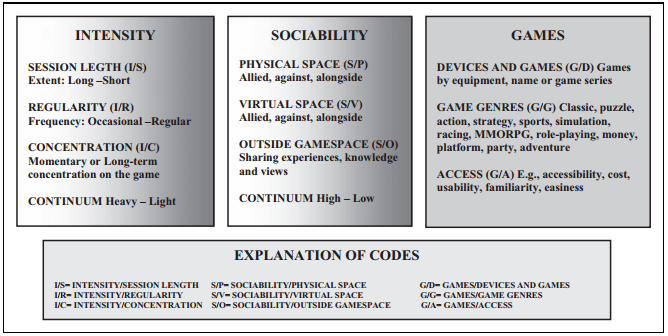
\includegraphics[width=\textwidth]{Figures/kallio-gaming-mentalities-model}
	\caption{The three components of gaming mentalities, as seen in Kallio et al. \cite{kallio2011gamermentalities}}
	\label{fig:kallio-gamer-mentalities-model}
\end{figure}

The social mentality profiles identified by Kallio et al. are of \emph{"quite light"} intensity, very high sociability and their choice in games focus on access to the games. The casual mentality profiles have variable intensity, low sociability and their choice in games focuses primarily on the device and access. The committed mentality profiles have \emph{"heavy"} intensity, high sociability and their choice in games focuses primarily on the genre. Each of the groups of profiles consist of three profiles with different, although similar, values for the various metrics defined in the model. \advice{Is this paragraph (or even source) really of any use here?}

Hamari \& Tuunanen \cite{hamari2014playertypes} used this and other papers to identify a total of five \emph{"key dimensions pertaining to motivations of play/orientation of the player"}: \emph{Achievement}, \emph{Exploration}, \emph{Sociability}, \emph{Domination} and \emph{Immersion}.

In this project, we will use the five archetypal player types \emph{Achieving}, \emph{Exploring}, \emph{Socializing}, \emph{Dominating} and \emph{Immersing}, where each of them is \emph{more concerned with} their respective dimension of the game than the four others, rather than \emph{entirely focused on} only that aspect. That is, for a \emph{Socializing} player, the social aspect of the game is more important than any other aspect, but they may still have varying interest in the other four dimensions.

\todo{Reference these types other places in the report, especially in success factors chapter}

\section{Motivation in Gaming}
\label{sec:motivation-in-gaming}

When considering motivation, we typically distinguish between \emph{intrinsic} and \emph{extrinsic} motivation. \emph{Extrinsic motivation} is motivation from outside sources such as the promise of receiving rewards for successful completion of a task, or punishment should one fail to complete the task. \emph{Intrinsic motivation} on the other hand refers to motivation coming from within, where performing a task is in itself personally rewarding, either because it is fun, exciting, enjoyably challenging or a variety of other positive emotions.

Malone \cite{malone1981toward} proposes challenge, fantasy and curiosity as the primary factors of intrinsic motivation in gaming. Looking back at the player types established in Section \ref{sec:player-types}, the Achieving and Dominating players have challenge as their primary intrinsic motivator, while the Immersing player is motivated by fantasy and the Exploring player is motivated by curiosity. The Socializing player's main source of motivation is not related to the game itself.

While some studies suggest that extrinsic motivation can conflict with and undermine intrinsic motivation (see for example Benabou \& Tirole \cite{benabou2003intrinsic}, Lepper \& Henderlong \cite{lepper2000motivation}), extrinsic rewards are common in video games. By progressing or performing difficult tasks in games, players unlock new types of items or characters, receive powerful items or abilities, in-game currency, cosmetic modifications to their avatar, recognition from other players from being placed in a hall of fame or leader board of some kind, or any number of other rewards. For some, these rewards do indeed remove the fun - the intrinsic motivation - from the game, turning it into a chase for the next reward. For others, however, these rewards help bring back the fun they were no longer able to find, enjoying the game more when being rewarded.

In a market with hundreds of thousands of games and players with short attention spans, however, extrinsic rewards for small feats has become common. To keep players active, they are awarded for doing a minimal amount of effort every day through daily reward systems, often of the form \emph{First X of the day}. For some developers, this is the final step for the game: a last resort to keep players playing their game. For others, it is a means to bridge the gap until they can introduce new features.

\todo{Mention this especially in "reasons to quit - the grind"}

% Chapter - Current state of physical and mental health in society (western world?)
\chapter{Health and Gaming}
\label{chapter:lit-study-modern-health}
\lhead{Chapter \ref{chapter:lit-study-modern-health}. \emph{Modern Society and Health}}

This chapter looks at some previous research on the effect of gaming on physical and mental health.

\section{Physical Activity}
\label{sec:lit-study-physical-activity}

Obesity is becoming an increasing problem as the world is further urbanized, and increasing physical inactivity is an important factor in the trend (Anderson \& Butcher \cite{anderson2006childhood}, Malik et al. \cite{malik2013global}, Uauy et al. \cite{uauy2001obesity}, Wang et al. \cite{wang2011health}). The World Health Organization (WHO) \cite{WHOobesity} report that worldwide obesity has more than doubled since 1980, with 39 \% of adults aged 18 years and older being overweight, and 13 \% being obese. To combat this, they recommend adults do \emph{"at least 150 minutes of moderate-intensity aerobic physical activity throughout the week"}, while children should do 60 minutes per day \cite{WHOphysical}. Janssen \& LeBlanc \cite{janssen2010systematic} performed a review of previous studies on \emph{"the relation between physical activity, fitness, and health in school-aged children and youth"}, and made similar recommendations based on these.

To motivate people to participate in physical activity, an emerging game trend in the last decade have been so-called \emph{exergames}. Whitehead et al. \cite{whitehead2010exergame} describe exergames as \emph{"video games that provide encouragement to exercise, particularly for an audience that may be reluctant to engage in the more traditional forms of exercise"}, further stating that \emph{"Exergames are a commonly accepted method of encouraging more physical activity to promote better health for those with high levels of sedentary screen time"}. Peng et al. \cite{peng2011playing} found that playing exergames were successful in increasing heart rate, oxygen consumption and energy expenditure to levels similar to those of traditional physical activities, and that they can \emph{"facilitate light- to moderate-intensity physical activity promotion"}.

\section{Mental Health}
\label{sec:lit-study-mental-health}

The WHO \cite{WHOdepression} estimate 350 million people worldwide suffering from depression, and the Anxiety and Depression Association of America (ADAA) \cite{ADAAanxiety} reports 18 \% of the US population suffering from anxiety disorders. These are serious disorders, and can in the worst case lead to suicide, yet less than half of those suffering, and in some countries fewer than 10 \% \cite{WHOdepression}, receive treatment for their condition.

Studies show that exercise can have a positive effect on depression, moderately to significantly reducing symptoms (Babyak et al. \cite{babyak2000exercise}, Dunn et al. \cite{dunn2005exercise}, Cooney et al. \cite{cooney2014exercise}), while Petruzzello et al. \cite{petruzzello1991meta}, Salmon \cite{salmon2001effects}, and Ströhle \cite{strohle2009physical} also found potential for a positive effect on anxiety disorders.

Rosenberg et al. \cite{rosenberg2010exergames} found potential for exergames to significantly improve symptoms of depression among elderly, and Brox et al. \cite{brox2011exergames} used exergames to a combined effect of increasing physical activity and decreasing loneliness among elderly.

\todo{Coulton et al. (Harnessing Player Creativity ...) about social in AR games?}


% Chapter - Similar games
\chapter{Similar Games}
\label{chapter:lit-study-similar-games}
\lhead{Chapter \ref{chapter:lit-study-similar-games}. \emph{Game Types}}

This chapter looks at some games that are relevant to compare with Pokémon GO, for the most part miscellaneous pervasive games. Some games are more similar than others, but all of them share some aspect with Pokémon GO, be it the play style, game concepts or the device used to play.

\section{Ingress}

Ingress is a location-aware, augmented reality game for Android and iOS phones. Like Pokémon GO, it was developed by Niantic Labs while it was a part of \emph{Google}. It was first officially released on Android in December 2013, and is considered by many to be the precursor to Pokémon GO. In an interview in October 2013 \cite{gamasutraBadger}, the product manager of Ingress stated that \emph{"Our vision for this, from Niantic Labs, is really to build a platform and to help other game studios, other developers, build similar types of geo-games on top of this infrastructure"}. Not only was it one of the first augmented reality games for mobile devices to enjoy commercial success, but it also laid the groundwork for more games to come. \nice{Maybe something about popularity compared to PoGo}

The game narrative explains that so-called \emph{Exotic Matter (XM)} is spreading across the world from \emph{Portals}, and have been linked to an unseen alien race called \emph{the Shapers}. The players choose between two teams: the \emph{Enlightened}, who embrace the alien influence, and the \emph{Resistance}, who wish to save the human race from their \emph{ingress} into our world. The portals and exotic matter are visible through the player's \emph{scanner}, which is the mobile device the game is installed on.

\begin{figure}[h]
	\centering
	\begin{subfigure}{0.45\textwidth}
		\centering
		
\includegraphics{Figures/ingress-logo}
		\caption{The Ingress logo}
	\end{subfigure}
	~
	\begin{subfigure}{0.45\textwidth}
		\centering
		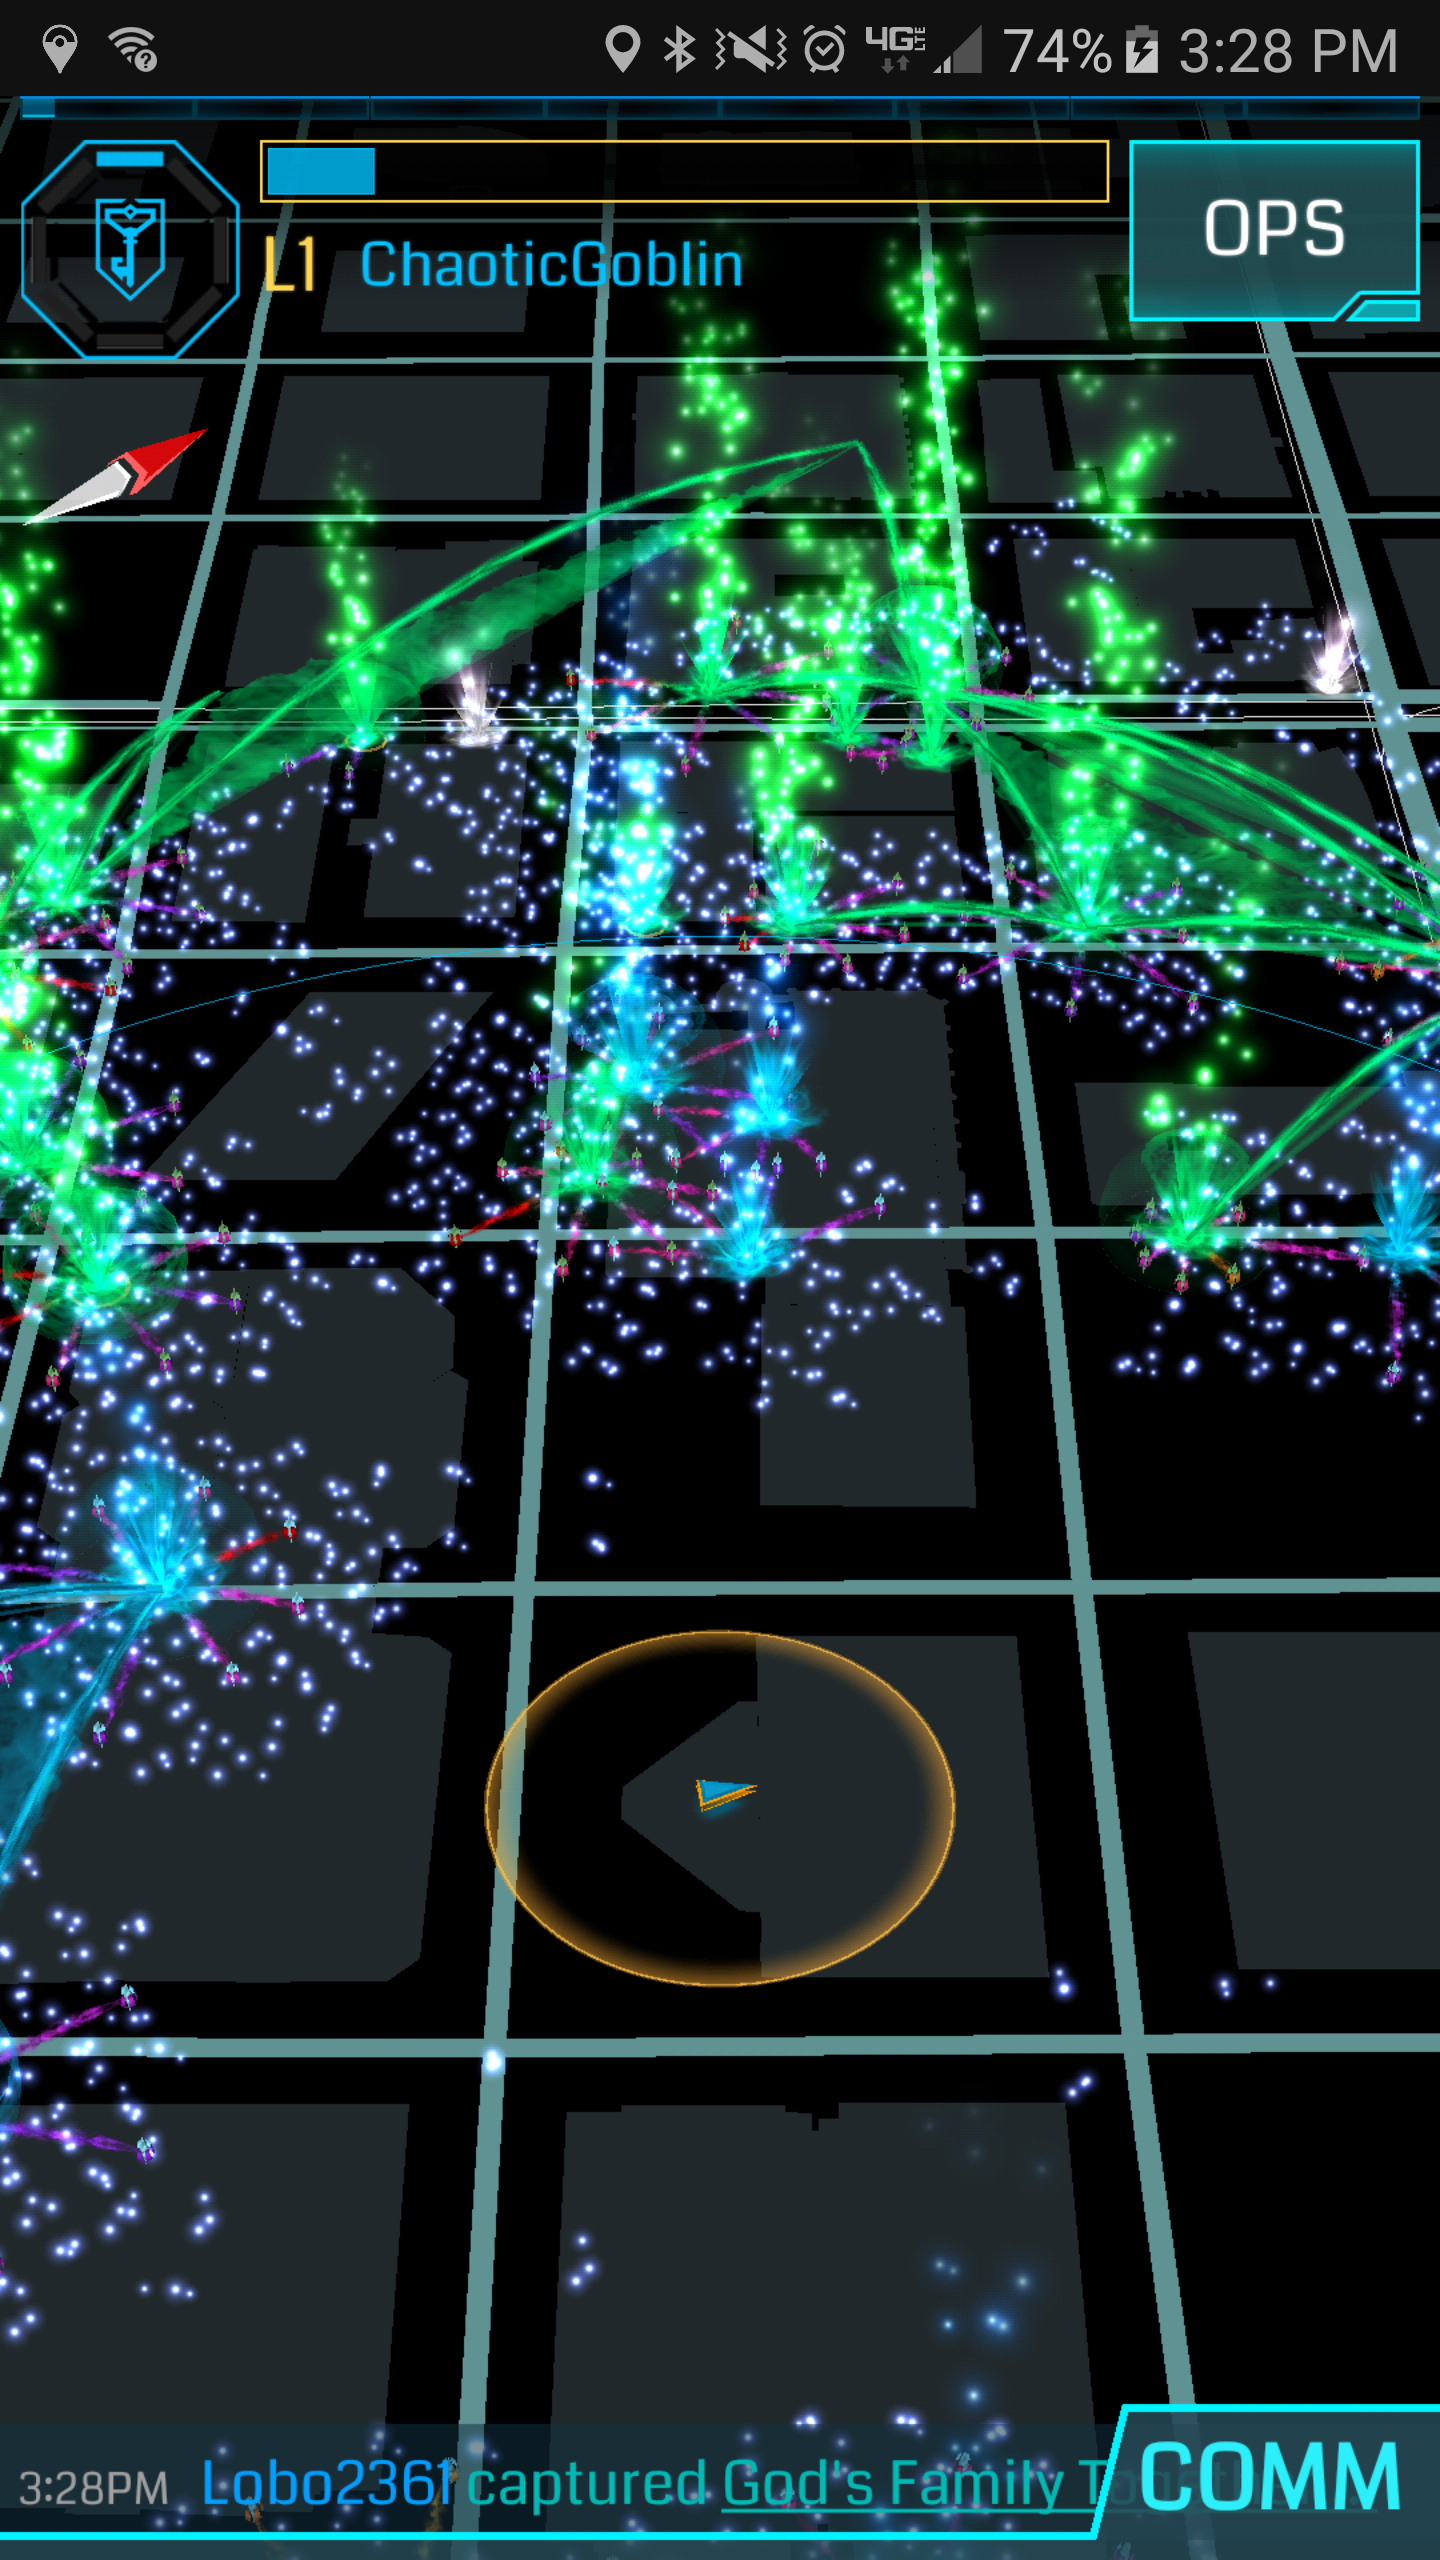
\includegraphics[height=3.2in]{Figures/chaoticgoblin-ingress-screenshot}
		\caption{A screenshot from the game, by Reddit user chaoticgoblin}
	\end{subfigure}
	\caption{Ingress}
\end{figure}

The game revolves around these portals, which players can \emph{hack} to retrieve items that help them claim these and other portals, while the XM they collect by moving around can be used to damage enemy portals. When a team is in complete control of multiple portals, players from that team can \emph{link} these portals to create a \emph{field}. Creating a field will claim the \emph{mind units} under the field for that team.

Portals in the game can be found at landmarks or points of interest, such as statues or buildings of note. Initially, the portals were based on \emph{"historical markers"}, but players could submit locations with descriptions to Niantic, and many of these were added to the game as portals \cite{mashableHanke}. Portal locations were also added later in conjunction with partnerships with various commercial chains such as \emph{Vodafone} \cite{auroraPromotion} or \emph{Jamba Juice}.

Progress in the game comes from performing actions, which yield \emph{action points (AP)} or earning \emph{badges} through achieving specific feats such as holding a friendly portal for a certain amount of time. The rewards for advancing in level is unlocking new, better items, and the only way to advance past level 9 (out of 16) is through earning badges.

Using Kiefer et al.'s \cite{kiefer2006systematically} game dimensions, the game is a \emph{strategy} more than anything else, requiring a solid plan if one wishes to have control over large areas. Although the game is referred to as an augmented reality game, using Kiefer et al.'s definitions, it is closer to a mixed reality game. XM is not perceptible in the real world, nor are the links or fields created. The portals are visible in the real world, but only in the capacity that they are real life objects, and this capacity does not depend on the game. Thus we have to argue that this is a \emph{mixed reality game}. If we ignore the XM, the game is spatially discrete, with game actions only taking place around portals. The collection of XM, however, is spatially continuous, as it can and will be collected mostly anywhere a player goes with the game open. The game is temporally continuous, with actions taking place at any time, although the game restricts the number of actions that can be taken on the same portal in a given time span. \emph{Anomalies}, special events inside and outside the game, take place at specific times, being temporally discrete.

\todo{f2p with in-game store and partnerships}

\section{Field Trip}

Another application developed by Niantic is Field Trip. It is not really a game in the way that most people think about games. It does not have rules, goals or other players. It is simply a tool that assists you in exploring. The app encourages you to explore by walking off in any arbitrary direction. When you get close to somewhere interesting, it notifies you. You can set preferences for what type of locations you are interested in, such as \emph{Architecture}, \emph{Historic Places \& Events} or \emph{Cool \& Unique}, and it will ignore other types of places while more frequently notifying you of these types of places.

\begin{figure}[h]
	\centering
	
\includegraphics[width=\textwidth]{Figures/fieldtrip-logo}
	\caption{The Field Trip logo}
\end{figure}

While the application is not a traditional game, it is worth mentioning not only because of its affiliation with Niantic, but because of its integration with Google's augmented reality device \emph{Google Glass}. With Field Trip, the Glasses show you \emph{cards} of the locations you encounter overlaid over what you usually would see, right in front of your eyes without requiring you to look at your phone or a similarly carried device.

Field Trip is also relevant in the way it encourages physical activity by suggesting you walk off in a random direction to explore, rather than find specific places before going out and traveling directly to them, something that often involves less physically exerting modes of transportation. Given that you are exploring somewhere with locations within your field of interest registered in Google's databases, Field Trip rewards you for your (potentially unintended) exercise with new, possibly exciting locations. These features resemble those of some exergames, motivating "players" to exercise through untraditional means.

\section{Geocaching}

Geocaching is a popular family activity game similar to the sport \emph{orienteering}. It is a game played with real life objects, but uses a mobile application to register the location of the items. The application lets you see a map of caches in an area, register your findings and make lists for a planned session. The caches are containers placed at any location, and are typically hidden somewhere clever in this location. The containers contain a logbook which the finder signs with their codename and time they found the cache, while some larger caches also contain trinkets or items that players can trade for one of their own items. Some caches require that you solve puzzles in the app before its exact coordinates are revealed to you.

\begin{figure}[h]
	\centering
	\begin{subfigure}[t]{0.5\textwidth}
		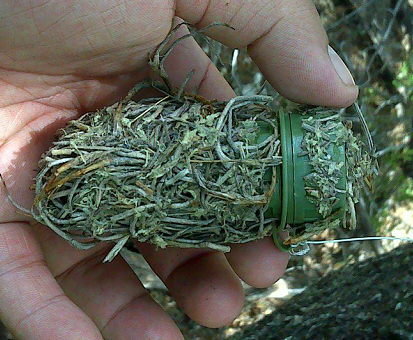
\includegraphics[height=2.5in]{Figures/chaoticgoblin-geocache-covered}
		\caption{Cache covered in natural camouflage}
	\end{subfigure}
	~
	\begin{subfigure}[t]{0.4\textwidth}
		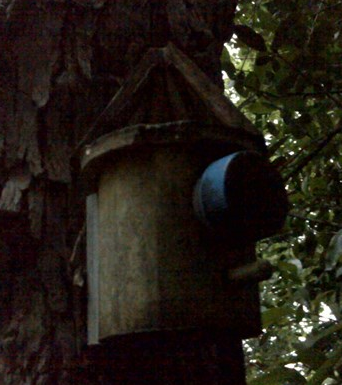
\includegraphics[height=2.5in]{Figures/chaoticgoblin-geocache-birdhouse}
		\caption{Cache hidden in birdhouse}
	\end{subfigure}
	~
	\begin{subfigure}[t]{\textwidth}
		\centering
		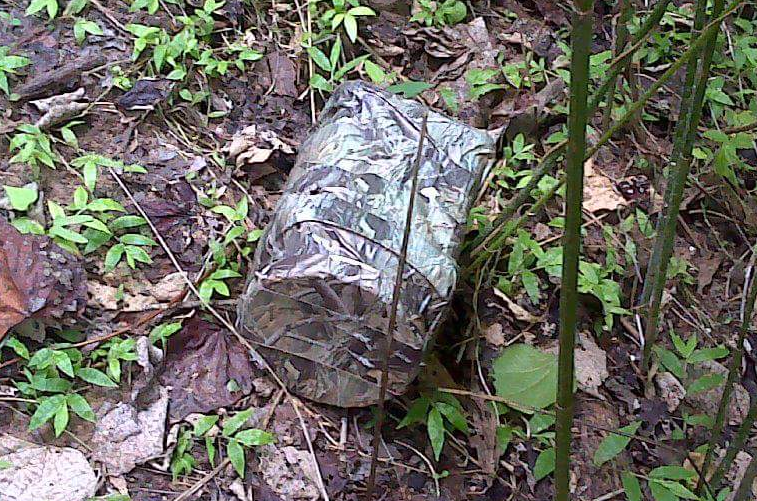
\includegraphics[height=2.5in]{Figures/chaoticgoblin-geocache-camo}
		\caption{Cache in camouflage-taped container}
	\end{subfigure}
	\caption{Clever hiding spots for geocaches (by Reddit user chaoticgoblin)}
	\label{fig:geocache-spots}
\end{figure}

Going back to Kiefer et al.'s \cite{kiefer2006systematically} dimensions for location-based games, Geocaching is primarily an item hunt game, and is in fact used as the most prominent example of one in their paper. Figure \ref{fig:geocache-spots} shows three clever hiding spots for caches found by Reddit user \emph{chaoticgoblin}, intended to make the player really have to search to find them. However, with the addition of caches that require you to solve puzzles to reveal their coordinates, Geocaching also gains aspects of a puzzle game. It is a pure location-based game, using localization technology solely to inform players of the location of the physical items, items that have no virtual equivalent. While caches technically can be placed anywhere, the actual locations of caches, where game events take place, are discrete and fairly static. Creating and placing a new cache can be done anywhere, but once placed, the location is discrete. Thus we classify Geocaching as spatially discrete. The game can be played at any time, and is thus temporally continuous.

\todo{f2p, makes money through partnerships (they offer different packages) and premium features}

\section{Zombies, Run!}

Zombies, Run! is an exergame for Android and iOS devices. First released in 2012, it has added a new \emph{season} of content each year since, and now has 200 missions to play through. Within two weeks of its release, it was the highest grossing app in the Health \& Fitness category in the iOS App Store, and now has a million players.

\begin{figure}[h]
	\centering
	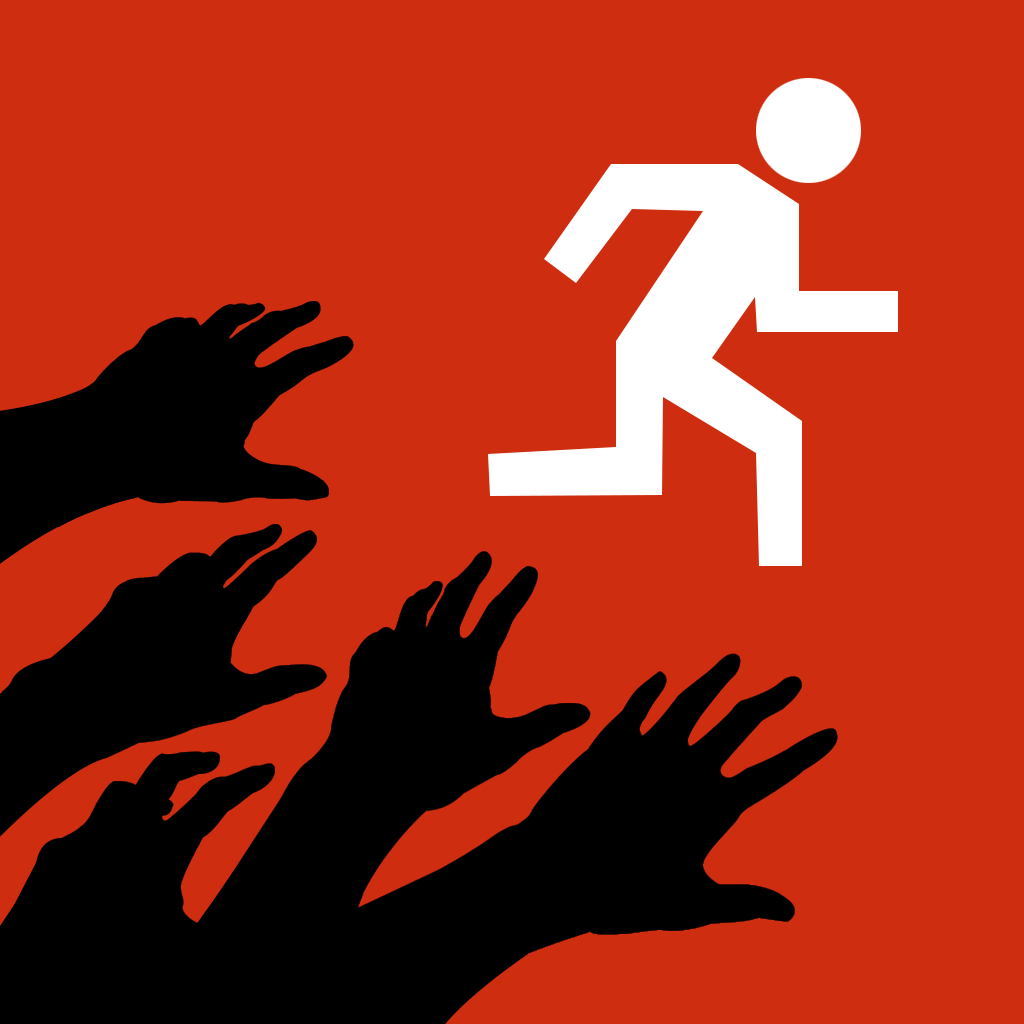
\includegraphics[height=2in]{Figures/zombies-run-logo}
	\caption{The \emph{Zombies, Run!} logo}
\end{figure}

The game narrative places the player in a post-zombie-apocalyptic world, and you are one of few survivors. By going out to run, you'll collect supplies used to build up a base for you and fellow survivors. The game features 200 missions that are narrated mini-stories that drive the plot forward as you build up your base, playing audio clips in between your own music as you run. During your run, it is possible for zombies to appear and chase you, requiring an increased pace. Should you fail to increase your pace and outrun them, they will catch up to you and any supplies you have collected will be lost.

The game uses the device screen minimally to select missions and viewing and sharing your progress between runs, while the game experience is presented through audio. There are no visual augmentations of reality, but the game uses audio clips to perceptibly augment a run. When being chased by zombies, their groans can be heard closing in if you do not run quickly enough, and their distance to you can be felt through the volume and intensity of their sounds. The game also plays a heartbeat in your ears, intended to imitate your own as you run. Southerton \cite{southerton2013zombies} performed an \emph{autoethnography} noting her experiences with the game, and found the heartbeat in particular to add high levels of immersion by adding a sense of urgency, but only during the other audio clips presented by the game.

\begin{figure}[h]
	\centering
	\begin{subfigure}{0.45\textwidth}
		\centering
		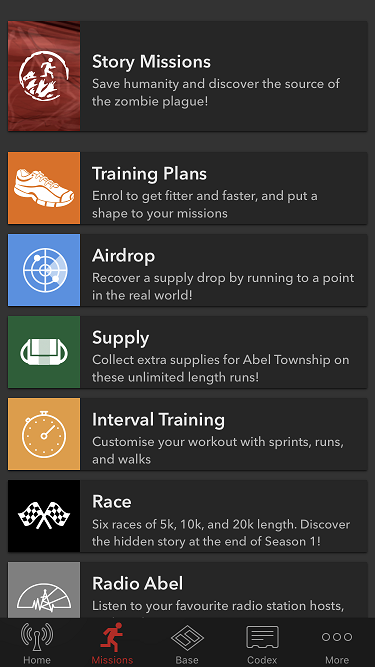
\includegraphics[height=3in]{Figures/zombies-run-activities}
		\caption{Activities available}
	\end{subfigure}
	~
	\begin{subfigure}{0.45\textwidth}
		\centering
		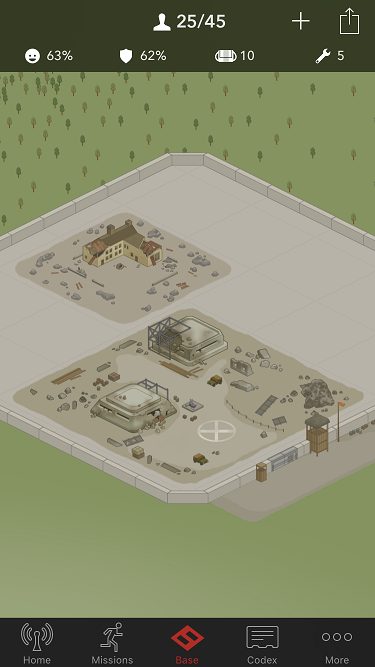
\includegraphics[height=3in]{Figures/zombies-run-base}
		\caption{View of the player's base}
	\end{subfigure}
	\caption{Screenshots of \emph{Zombies, Run!}}
\end{figure}

With basis in Kiefer et al.'s \cite{kiefer2006systematically} paper, Zombies, Run! is a location-based game in that it uses GPS technology to track the player's movements in order to progress in the game by collecting supplies and to escape zombies. It also allows the player to choose a location on a map, and will generate a mission tailored to the distance to that location, called an \emph{Airdrop}. We classify Zombies, Run! as an augmented reality game, with virtual elements (zombies) perceptible in the real world through audio. The game is closest to a chase game, as outrunning the zombies is vital to game progress. The game progresses continually as the player moves, as long as they are on a mission, and a mission can be started at any time. Thus we classify the game as spatially and temporally continuous.

While the game is an exergame in the true sense of being a game with the sole purpose of encouraging physical activity, or more specifically aerobic exercise, the actual impact of the exercise it encourages has been debated. Halushak, an experienced runner, noted in her experience with the game that because of the sparse zombie attacks and high requirement to escape them that the game is more about exercising the players' imagination than to push them to their limits. Halushak's reasoning for this is that the player must increase their pace by at least 20 \% to escape, which is difficult when already running at a quick pace, encouraging an overall lower pace if one wants to be able to escape. Higgins \cite{higgins2016smartphone} in a review of smartphone apps for increasing patients' health and fitness recommended the game for \emph{"healthy patients wanting to start basic aerobic exercise"}, but not any other groups of patients. Other studies (Cowdery et al. \cite{cowdery2015exergame} and Direito et al. \cite{direito2015apps}) performed with the app showed that the physical impact was limited, but that players using these apps were more likely to be motivated to continue their exercise after the control periods.

\todo{Used to be purchaseable, now f2p with money from premium features and entry to special events}

\section{Munzee and Stolpejakten}

Munzee (a stylized version of the German word for \emph{coin}) is an scavenger hunt/item hunt game similar to Geocaching, using QR codes and GPS location to register captures as opposed to the physical hidden caches of Geocaching. As in Geocaching, \emph{Munzees} are deployed by players by registering a QR code in the app and placing a waterproof sticker with the code on it in a location of their choosing, which they then register to a map. Munzees are found all over the world, with at least one Munzee present on every continent - including Antarctica \cite{munzee}. Capturing a Munzee awards points to the player who made the capture as well as the player who deployed it.

Stolpejakten (meaning \emph{The Pole Hunt} in Norwegian) is a Norwegian game with a similar concept to Munzee, but instead of stickers attached to poles and other objects, special poles with QR codes attached are placed as markers for the game. The game is marketed as an exergame, with the goal of getting people of all ages and physical conditions active and providing a means of exploration for those who wish to get to know their local community better. They are color coded according to four levels of difficulty, where the \emph{green} poles are the easiest and are reachable by bicycle and wheelchair, and the \emph{black} poles are difficult and require a serious effort in reaching. Capturing a pole gives the user a ticket in a raffle held in the county the pole is located, sponsored by local businesses. Capturing more poles awards more tickets, increasing their odds of winning good prizes such as concert tickets, festival passes or three-course meals at good restaurants.

Both of these games share the two of the same game dimensions as Geocaching, in that they are pure location-based games and are spatially discrete and temporally continuous. They are arguably also item hunt games, Munzee more so than Stolpejakten, as the \emph{Munzees} are much smaller than the poles placed in Stolpejakten. Neither of the games share the puzzle game aspect of Geocaching.

\todo{Both f2p - Munzee offers partnerships and sells Munzees, Stolpejakten rents out infrastructure to local organizers and sell memberships to local clubs}

\section{Run an Empire}

Run an Empire is a social exergame where players compete to claim territory for their \emph{empire} through running or jogging. The map is split into \emph{hexes} (hexagonal tiles), and running across a hex stakes a claim to that hex. If your claim is stronger than all other players' claim to the hex, it will be added to your empire. You can strengthen your claim by running across the same hex on another run, and the stronger your claim, the more difficult it will be for intruders to take over your empire. Having more hexes in your empire grant a higher position on the leaderboards. There is both a global leaderboard and a social leaderboard, where the social leaderboard lists the players you are following in the game.

The game focuses on strategy rather than catering only to those of superior physical ability, making the game available and enjoyable for all players. They enable this by limiting each run to one hour, and only allowing one run per 24 hour period. New players are also accommodated by a limit to the strength of a player's claim to a hex, and \emph{tile decay} ensuring that as time passes, a claim weakens if it is not strengthened through active play. The limit also acts as an incentive to expand your area with new routes when your claim to one area is near its limit, an incentive that is further strengthened by the generation of gems randomly on the map when you start a new run. These gems can be used to buy certain items in the game to upgrade your empire. Players also earn coins by running, which encourages play even if the surrounding area is strongly held by an opponent, as coins can be stolen from opponents. These coins, like the gems, can be used to purchase items, and act as secondary points to show a player's achievements over time.

Using Kiefer et al.' game dimensions \cite{kiefer2006systematically}, the game is a mixed reality location-based game, with virtual objects on the map that are not perceivable outside the virtual game environment. It is a strategy game rather than a chase game for the reasons described above, and requires good planning to most efficiently expand your empire. The game area is continuous, and while you can start your first run at any point, the restrictions to length and frequency of runs makes the game temporally discrete. Thus it would seem that Run an Empire is a spatially continuous and temporally discrete game, the class that Kiefer et al. at the time were unable to discover.

\todo{Make money through sale of cosmetic items and }

\section{The Walk}
\todo{Story-driven audio AR}

\section{Mobile games}
\todo{Some examples of casual mobile games (e.g. Angry Birds, Candy Crush, Temple Run)}


% Chapter - More about Pokémon and Pokémon GO
\chapter{Pokémon}
\label{chapter:lit-study-pokemon-go}
\lhead{Chapter \ref{chapter:lit-study-pokemon-go}. \emph{Pokémon GO}}

\section{Pokémon Franchise}
\todo{Short introduction to the Pokémon franchise, some terms and the different games?}

\section{Pokémon GO In-Depth}
\label{sec:pokemon-go-in-depth}
\todo{Description of every feature of Pokémon GO, and the technology it uses. Also describe game type based on theory from Chapter \ref{chapter:lit-study-game-theory}}

\section{Pokémon GO in the Media}
\todo{Mention and cite some articles about Pokémon GO. } \advice{Are Norwegian articles fine?}
 

\part{Player Study}
\label{part:player-study}
% Chapter 3

\chapter{Introduction to the Player Study}

\label{chapter:player-study-introduction}
\lhead{Chapter \ref{chapter:player-study-introduction}. \emph{Player Study - Introduction}}

% Section 1 - Survey distribution
\section{Survey Distribution}

The survey was distributed in a Norwegian and an English version, and in multiple phases. After the first phase, some questions were adjusted, and a missing question regarding weight loss and perceived improvement on physical health was added. The final version of the survey can be found in Appendix \ref{appendix:survey}.

The first phase of distribution took place at a large Pokémon Go event in \emph{Frognerparken} in Oslo, Norway, a large sculpture park and popular destination for Pokémon Go players due to the high density of Pokéstops and spawns. The survey was available online via an easily accessible custom URL from a known link shortener, leading to the Norwegian version. Single players and groups of players were approached over the span of about two hours, given a short introduction to the project and asked whether they would be willing to respond to the survey. Given a positive response, they were handed a note with the URL. Extra effort was made to reach out to players in the following categories: Young children (15 or below), parents playing with children, and players above 40. This was done in an attempt to reach the broad spectrum of ages participating, even though the bulk of players are between the ages of 20 and 35. \todo{Should I mention the number of responses that (likely) originated from here?}

In the second phase, the survey was distributed on \emph{Facebook}. A post explaining the project and an encouragement to respond despite the length of the survey, along with links to both versions, was shared in each of the four largest Norwegian Pokémon Go groups (\emph{Pokémon GO: Norway}, \emph{Pokemon Go Norge}, \emph{Pokémong GO - Oslo \& Akershus} and \emph{Pokémon GO Trondheim}), as well as personally. It was then re-shared by several people to their local Pokémon GO groups or their personal friends and followers. \todo{Could mention an estimate of the amount of people reached through these groups, and the amount of responses it yielded?}

The third phase involved sharing the survey on the popular internet forum \emph{Reddit}. Here it was shared in two \emph{subreddits}, sub-forums on the larger site with their own dedicated communities. The first subreddit was \emph{/r/PokemonGo}, the main community for people interested in the game in general. The second, \emph{/r/TheSilphRoad}, is a community devoted to research on all things related to Pokémon GO.

In addition to the three main phases of distribution, people encountered playing or talking about the game at any time were approached and asked to participate throughout all of September.

In early December, the respondents who had left contact information were contacted with a short follow-up survey, seen in Appendix \ref{appendix:followup}. Those who had left comments of note separating them from the other respondents were also asked about these points of interest. This second questionnaire was an attempt to gather information on the longevity of the game, some clarifications of questions from the original survey and a question about spending money in the game. 

\todo{Perhaps include a figure of the distribution of link clicks?}

% Section 2 - Demographics
\section{Demographics}

The survey collected data on the demographics of its respondents, including the age, gender and the country in which most of their playing occurred. The recorded nation is assumed to be their country of residence in most cases. A total of 2190 responses were recorded with demographic data.

Out of everyone who responded, 1244 (slightly below 57 \%) were male and 946 were female. Figure \ref{fig:respondents-age-histogram} shows a histogram of the ages of all respondents, ranging from 5 to 67 years old, with the largest number of respondents (176) being aged 25. Respondents have also been divided into seven different age groups, show in Table \ref{tbl:survey-age-distribution}. Note that the total percentages are rounded, and rounding errors cause the total to sum up to 101 \%.

\begin{figure}[h]
	\centering
	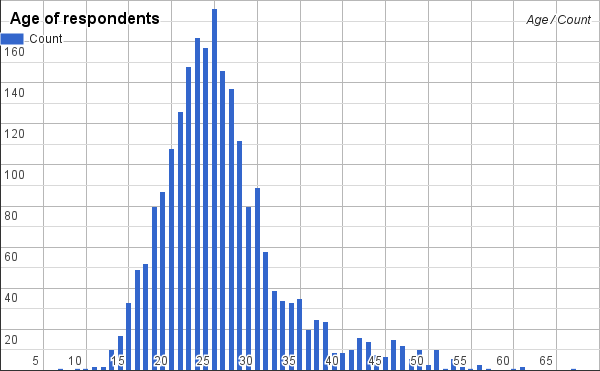
\includegraphics[width=\textwidth]{Figures/age-histogram}
	\caption{A histogram of the ages of the respondents}
	\label{fig:respondents-age-histogram}
\end{figure}

\begin{table}[h]
	\centering
	\caption{Age distribution of survey respondents}
	\label{tbl:survey-age-distribution}
	\begin{tabular}{|l||c|c|c|c|c|c|c|}
		\hline
		&\textbf{18-} & \textbf{18-21} & \textbf{22-26} & \textbf{27-32} & \textbf{33-40} & \textbf{41-50} & \textbf{50+}\\
		\hline\hline
		
		\textbf{Male} & 120 & 247 & 434 & 284 & 108 & 37 & 14 \\
		\hline
		
		\textbf{Female} & 48 & 154 & 355 & 231 & 81 & 64 & 14 \\
		\hline
		
		\textbf{Total} & 168 & 401 & 789 & 515 & 189 & 101 & 28 \\
						& 8\% & 18\% & 36\% & 24\% & 9\% & 5\% & 1\%\\
		\hline
	\end{tabular}
\end{table}

\todo{Mention the results normalized for responses per gender: More popular among males in the younger categories and females in the older categories (even in the middle). Matches observations of groups of young boys playing but few young girls, and maybe a reference to older women and walking groups}

The results contained 1192 responses stating Norway as their main location for playing. Because the survey was distributed in Norwegian Facebook groups, but not in local communities for other countries, Norway has been excluded from the following \todo{table/figure}, which shows the distribution of players per country for the remaining 998 respondents.

\todo{Include table or figure showing the countries of respondents}

The survey also asked for the main occupation of each respondent, with four categories available: employed, unemployed, higher education (e.g. university or college) and lower education (e.g. high school or middle school). The following table again shows the distribution between these categories. \todo{This data probably isn't very relevant and could possibly be removed.}

\begin{table}[h]
	\centering
	\caption{Distribution of survey respondents across occupations}
	\label{tbl:survey-occupation-distribution}
	\begin{tabularx}{\textwidth}{|l|l|X|X|}
		\hline
		\textbf{Lower education} & \textbf{Higher education} & \textbf{Employed} & \textbf{Unemployed}\\
		\hline\hline
		
		219 & 747 & 1056 & 169\\
		\hline
	\end{tabularx}
\end{table}

% Section 3 - Mapping to research questions
\section{Survey and Research Questions}

The purpose of the survey was to collect data to answer the research questions presented in Chapter \ref{chapter:research-questions}. This section will provide a mapping between the questions of the survey and the research questions each of them aim to answer. It should be noted that in addition to the listed questions, the survey included a comment section at the end where respondents could provide any additional info they did not find a proper place for, and these comments have also been used to evaluate the research questions.

\todo{Consider using tree graphs instead of tables to illustrate}

The first research goal, examining the success factors of Pokémon GO as seen in Section \ref{rg1}, was decomposed into five research questions, \ref{RQ1.1} through \ref{RQ1.5}. Table \ref{tbl:rg1-survey-questions} shows the survey questions relevant for this research goal and the research questions each of them help answering.

\begin{table}[h]
	\caption{\emph{What are the main factors that made Pokémon GO successful?} Survey Questions}
	\centering
	\label{tbl:rg1-survey-questions}
	\begin{tabularx}{\textwidth}{|X|l|}
		\hline
		\textbf{Survey question} & \textbf{Research questions}\\
		\hline\hline
		
		Which of the following factors influenced your decision to start playing Pokémon Go? & \ref{RQ1.1}\\
		\hline
		
		Which of the following game features do you use? & \ref{RQ1.2}\\
		\hline
		
		If you have previously played any location-based or augmented reality games, what did you like about them and what did you not like about them? How does Pokémon Go compare on these points? & \ref{RQ1.3}\\
		\hline
		
		If you have previously played any other casual mobile games, what did you like about them and what did you not like about them? How does Pokémon Go compare on these points? & \ref{RQ1.3}\\
		\hline
		
		If you have previously played any other Pokémon games, what did you like about them and what did you not like about them? How does Pokémon Go compare on these points? & \ref{RQ1.4}\\
		\hline
		
		If you are no longer playing, when and why did you stop? If you are still playing, but have greatly reduced the amount you play, when and why did this happen? & \ref{RQ1.5}\\
		\hline
	\end{tabularx}
\end{table}

The second research goal, evaluating the physical health effect of playing Pokémon GO as seen in section \ref{rg2} was decomposed into six research questions, \ref{rq-physical-activity-amount} through \ref{rq-physical-risks}. Table \ref{tbl:rg2-survey-questions} shows the survey questions relevant for this research goal and the research questions each of them help answering.

\begin{table}[h]
\caption{\emph{What are the effects on physical health from playing Pokémon GO, and how much effort does it take to achieve this effect?} Survey Questions}
\centering
\label{tbl:rg2-survey-questions}
	\begin{tabularx}{\textwidth}{|X|l|}
		\hline
		\textbf{Survey question} & \textbf{Research questions}\\
		\hline\hline
		
		In an average week, how much time did you spend on physical activities (e.g. walking, running or biking) before you started playing Pokémon Go? & \ref{rq-physical-activity-amount}, \ref{rq-physical-high-low-comparison}\\
		\hline
		
		In an average week, how much time do you spend on physical activities since you started playing Pokémon Go? & \ref{rq-physical-activity-amount}, \ref{rq-physical-high-low-comparison}\\
		\hline
		
		If you spend more time on physical activities after you started playing Pokémon Go than before, what are the sources of this activity? & \ref{rq-physical-game-activities}\\
		\hline
		
		Have you lost weight or in other ways feel more healthy than before you started playing Pokémon Go? & \ref{rq-physical-weight-loss}\\
		\hline
		
		Have you skipped out on less healthy activities (e.g. going out to drink) that you otherwise would have engaged in due to playing Pokémon Go instead? If so, please specify. & \ref{rq-physical-unhealthy-habits}\\
		\hline
		
		Have you trespassed or otherwise gone into areas you shouldn’t be because you were playing Pokémon Go? & \ref{rq-physical-risks}\\
		\hline
		
		Have you put yourself or others in dangerous situations because you were playing Pokémon Go? & \ref{rq-physical-risks}\\
		\hline
		
		Have you gotten into any accidents because either you or another involved party was playing Pokémon Go? & \ref{rq-physical-risks}\\
		\hline
		
		If you have put yourself or others in dangerous situations, or gotten into accidents, because of Pokémon Go, could you elaborate? & \ref{rq-physical-risks}\\
		\hline
		
		Have you neglected other areas of your life because you were playing Pokémon Go? & \ref{rq-physical-risks}\\
		\hline
	\end{tabularx}
\end{table}

The third research goal, evaluating the mental health effect of playing Pokémon GO as seen in section \ref{rg2} was decomposed into four research questions, \ref{rq-mental-social-activity-amount} through \ref{rq-mental-illnesses}. Table \ref{tbl:rg3-survey-questions} shows the survey questions relevant for this research goal and the research questions each of them help answering.

\begin{table}[h]
	\caption{\emph{What are the effects on mental health from playing Pokémon GO?} Survey Questions}
	\centering
	\label{tbl:rg3-survey-questions}
	\begin{tabularx}{\textwidth}{|X|l|}
		\hline
		\textbf{Survey question} & \textbf{Research questions}\\
		\hline\hline
		
		In an average week, during your spare time, how much time did you spend socializing with other people (in person, outside your home) before you started playing Pokémon Go? & \ref{rq-mental-social-activity-amount}\\
		\hline
		
		In an average week, during your spare time, how much time do you spend socializing with other people (in person, outside your home) since you started playing Pokémon Go? & \ref{rq-mental-social-activity-amount}\\
		\hline
		
		If you have increased the amount of time you spend socializing with people since you started playing Pokémon Go than before, what are the causes of this increase? & \ref{rq-mental-game-activities}\\
		\hline
		
		Have you talked to someone in person because of Pokémon Go that you otherwise would not have talked to? & \ref{rq-mental-relationships}\\
		\hline
		
		Have you made new friends through playing the game? & \ref{rq-mental-relationships}\\
		\hline
		
		Has playing Pokémon Go improved any of your existing relationships? & \ref{rq-mental-relationships}\\
		\hline
		
		Do you suffer from any mental illnesses? & \ref{rq-mental-illnesses}\\
		\hline
		
		If you suffer from a mental illness, do you feel that playing Pokémon Go has had a positive effect on your mental health? If yes, feel free to elaborate on how it has helped you & \ref{rq-mental-illnesses}\\
		\hline
	\end{tabularx}
\end{table}
% Chapter 4 - Player Study - Success factors

\chapter{Success Factors}
\label{chapter:player-study-success-factors}
\lhead{Chapter \ref{chapter:player-study-success-factors}. \emph{Player Study - Success Factors}}

This chapter examines the survey results in the context of determining the success factors of the game. The questions in Table \ref{tbl:rg1-survey-questions} and their answers are the main focus of this chapter, but relevant answers to other questions are also included.

\section{Results for Initial Interest}
\label{sec:success-factors-initial-interest-results}

To answer research question \ref{RQ1.1}, subjects were asked \emph{"Which of the following factors influenced your decision to start playing Pokémon GO?"}. Table \ref{tbl:initial-interest-options} shows the options that were supplied, as well as the number of respondents for each alternative. Subjects could choose more than one option, and the \emph{Other} choice allowed the respondent to describe other reasons.

\begin{table}[h]
	\caption{\emph{Which of the following factors influenced your decision to start playing Pokémon GO?} options and responses}
	\centering
	\label{tbl:initial-interest-options}
	\begin{tabular}{|l|c|c|}
		\hline
		\textbf{Option} & \textbf{Respondents} & \textbf{\% of total}\\
		\hline\hline
		Nostalgia or previous experience & 1507 & 70\\\hline
		Social media or internet forums & 764 & 35\\\hline
		Recommendations from friends/family & 738 & 34\\\hline
		Media coverage & 315 & 15\\\hline
		Official trailers/promotion & 308 & 14\\\hline
		The opportunity to get discounts or benefits & 9 & 0.5\\ because of Pokémon Go-related promotions && \\\hline
		Other & 165 & 8\\\hline
	\end{tabular}
\end{table}

The answers given for the \emph{Other} option were categorized, and Table \ref{tbl:initial-interest-other-categories} shows the categories with multiple answers, with the remaining responses grouped together as \emph{Miscellaneous}.

\begin{table}[h]
	\caption{\emph{Which of the following factors influenced your decision to start playing Pokémon GO?} Other categories}
	\centering
	\label{tbl:initial-interest-other-categories}
	\begin{tabular}{|l|c|c|}
		\hline
		\textbf{Category} & \textbf{Respondents} & \textbf{\% of Other}\\
		\hline\hline
		Pokémon & 43 & 26 \%\\\hline
		Exercise & 29 & 18 \%\\\hline
		Children/family & 26 & 16 \%\\\hline
		Ingress & 18 & 11 \%\\\hline
		Social & 7 & 4 \%\\\hline
		Technology & 6 & 4 \%\\\hline
		Fill outside time & 6 & 4 \%\\\hline
		Something to do & 5 & 3 \%\\\hline
		Real world & 5 & 3 \%\\\hline
		Trends & 4 & 2 \%\\\hline
		Gamer & 3 & 2 \%\\\hline
		Miscellaneous & 10 & 6 \%\\\hline
	\end{tabular}
\end{table}

The \emph{Pokémon} category are respondents who said they started playing simply because it was Pokémon. They consume any product related to the franchise, and would not let a Pokémon game go unplayed. These respondents are primarily around their twenties, and have to an extent grown up with Pokémon.

The \emph{Ingress} category are respondents who had previously played Ingress. Some active Ingress players were part of the Pokémon GO beta because of their participation, while others simply wanted to try another similar game. The \emph{Gamer} category are respondents who identify as gamers and picked up Pokémon GO because it was a new game, despite not having previous experience with either Pokémon or Ingress.

The \emph{Exercise} category are respondents who picked up the game as an exercise app, and wanted to use it as an excuse to walk more or a final push to get out and exercise, while the \emph{Fill outside time} are respondents who were already exercising or walking and wanted something to do during these activities.

The \emph{Children/family} category are respondents who either started playing because they wanted to spend time with their children or other family members who were already playing, or decided together with family members (significant others included) to start playing as a common activity. The \emph{Social} category are those who had similar goals with friends or who merely mentioned they started for the social aspect without specifying who they wished to be social with.

The \emph{Technology} category are respondents who were drawn to the game because of the technology used, be it augmented reality, GPS tracking or otherwise. The \emph{Real world} category are respondents who started playing because of the real world integration. They either wanted to find out what familiar locations had been turned into Pokéstops, or use the game to explore and find new and interesting locations. One subject in this category reported that they started playing because a sculpture they had made had been turned into a Pokéstop.

The \emph{Something to do} category are respondents who picked up the game just as something to do, either because they were bored at vacation or similar, or because they needed a distraction.

The \emph{Trends} category are respondents who started playing to take part in the cultural phenomenon and keep up with current trends.

\todo{Maybe add something about start time?}

\section{Analysis of Results for Initial Interest}
\label{sec:success-factors-initial-interest-analysis}

As expected, the Pokémon brand played a major role in spreading the game to such a vast number of players. 2164 respondents supplied a reason for downloading the game, and 1507 of them - almost 70 \% - listed \emph{Nostalgia or previous experience} as one of or the only reason they started playing. Releasing a Pokémon game that did not require any additional console (e.g. Nintendo DS) but could be played on the smartphone everyone was already carrying was all but guaranteed to be a success. However, not all games can be Pokémon games, so what other things did Pokémon GO do right that we can use to create other successful games? A little over 30 \% of the respondents did not list nostalgia as a reason, and while some of them may have had memories of watching or playing Pokémon but for some reason or other did not pick this choice, there were certainly players who had no previous experience or connection with Pokémon.

The opportunity to get discounts or benefits because of Pokémon GO-related promotions did draw a few players, but with less than 0.5 \% of the respondents listing this as a reason, it seems negligible. Those who responded within the \emph{Pokémon} category can be grouped together with the nostalgia responders and should thus be ignored as well.

308 respondents, or just over 14 \%, said they were affected by official trailers or promotional material. This shows that the advertisements \todo{(were there more than the Super Bowl ad?)} were helpful in creating interest in the game. While 14 \% is a relatively small portion compared to the numbers for the other responses, the more casual players who were not reached by the survey (see more in Section \ref{sec:problems-with-survey}) may have had a larger portion of players who were intrigued by the Super Bowl ad but who did not have much previous experience with Pokémon. \todo{Insert picture from the Super Bowl ad here.}

During the first few weeks following the release of the game, there was quite extensive coverage of the game in media all over the world. A little under 15 \% of respondents said that this media coverage affected their decision to start playing Pokémon GO, meaning it was slightly more effective than the official promotional material at building the player base, despite not an insignificant number of the articles posted were negative in their view \todo{(add some citations for negative articles)}. However, the media would not have covered the phenomenon to such a degree had there not already been a huge player base, but if one can succeed in spreading the game to a large enough number of players such that the media starts covering the game, it is not unlikely that one can achieve a similar growth of an additional 15 \% players \todo{(does this argument make sense?)}. Those who responded within the \emph{Trends} category can also be included in this group.

A combined 69 \% of respondents said they started playing because of either recommendations from friends or family or from reading about the game on social media or internet forums. Similar to the \emph{Media coverage} group, these groups required someone else to pick up the game before them, but a huge following is not required for this to have an effect, unlike what is necessary for media coverage to kick in. Thus it could seem that if one can successfully spread ones game to an initial group of players and the game is appealing enough, it can easily spread naturally via them.

Veteran Ingress players were part of this initial group for Pokémon GO, and almost 11 \% of those who listed other reasons were previous Ingress players who either had been granted beta access to Pokémon GO or started playing it because they were previously familiar with the games from the developer. This also indicates that if a developer already has a successful game (even if somewhat niche, like Ingress), it is possible to adjust some parts of the game and release a new one and gain an initial player base from those familiar with your previous games. This is what game developers have been doing for years, and is also in line with \todo{Kiefer et al. (insert citation, "Systematically Exploring Design Space ...)}.

The \emph{Children/family} and \emph{Social} categories are partly related to the idea of creating an initial player base and letting it grow through sharing, but they also highlight the importance of the social aspect of the game. One area where Pokémon GO succeeded is making the game very social, and it becomes more fun to play together with others, as shown by 20 \% of the \emph{Other} responses placing in these categories. Players enjoyed going out to play with their friends and family, having a purpose and something to do while socializing. More on this in Section \ref{sub:mental-health-social}. \todo{Add a note and citation for Coulton et al. (Harnessing Player Creativity ...) perhaps?}

The use of augmented reality technology and anchoring to the real world using GPS positioning also succeeded in attracting some number of players. About 7 \% of responses for the \emph{Other} option gave these areas as one of or the sole reason for playing. There still are not a large number of games using these technologies, and being one of the few that do allowed Pokémon GO to grab a market share by filling a hole. Some examples of other games with relative success in these areas were mentioned in Section \ref{sec:prestudy-ar-location-pervasive-games}, but there should still be room for more games in this category, and new, successful games could be created by changing some parameters of the Pokémon GO formula, as described in \todo{Kiefer et al. (ok with another citation of this only two paragraphs after the previous?)}.

Another category related to real world integration is \emph{Fill outside time}. The respondents in this category take advantage of the location-based aspect of the game, where the game progresses simply by moving around. They were looking for an activity to fill the time they were already spending outside, either walking somewhere (e.g. to work, public transit etc.) or exercising, and a game that does not require their constant attention and actually progresses based on the activity they were already performing is a better fit than most other mobile games.

Even though Pokémon GO is not marketed as an exercise app, over 17 \% of respondents who chose the \emph{Other} option said they started playing the game with that exact purpose. The location-based gameplay serves as motivation to get up and out and to move around. With overweight being an increasing problem and sedentary lifestyles becoming increasingly common, we are frequently reminded by health institutions of the importance of physical activity. While most are aware that it is important to be physically active, many struggle with motivation. Not only being able to combine exercise with something fun, but the game actually requiring players to move around to progress makes Pokémon GO the perfect motivation for many players. Other games have also used a similar recipe to success before, as discussed in Section \ref{sec:prestudy-ar-location-pervasive-games}.

The \emph{Something to do} and \emph{Gamer} categories can also be more or less ignored, because it is difficult \todo{(impossible?)} to say what will attract these players to your game over another one. The \emph{Gamer}s are likely to pick up any game they stumble upon, and the quality of the game will determine whether or not they will stick with the game. The respondents in the \emph{Something to do} category will similarly start any activity in an attempt to find something that can keep their attention. The best one can do to capture these players is to simply get the game as much exposure as possible to increase the odds of being the first activity or game they happen upon, and make sure the game is good enough to keep their attention. In the \emph{Miscellaneous} category are respondents whose reasons have too small of a sample size to draw any conclusions from.


\section{Important Features}
\label{sec:success-factors-features}

\todo{What features do the players like and use, comparing to other games}


\section{Results for Dwindling Interest}
Despite launching as a soaring success, the Pokémon GO bubble also burst relatively quickly. Player numbers started dwindling near the end of July as seen in Figure \ref{fig:player-numbers}, and by mid-August it had lost around 80 \% \todo{(check the number and get citation here)} of its active player base. This section and the following attempts to answer research question \ref{RQ1.5} and determine why Pokémon GO all but faded away so quickly.

\todo{Insert figure of global player numbers}

Table \ref{tbl:still-playing} shows the distribution of responses for the question \emph{"Are you still playing?"}. Not surprisingly, less than 3 \% of the responses said they had already quit playing, as those who have quit are for the most part no longer following Pokémon GO groups or forums even if they previously were. What is more interesting is that over 40 \% of respondents said they had reduced the amount of time they play compared to their peak. While we do not know how much they reduced their play time, we do know that they were playing less, and there had to be some reason for it.

\begin{table}[h]
	\centering
	\caption{\emph{Are you still playing?} survey question responses}
	\label{tbl:still-playing}
	\begin{tabular}{|c|c|l|}
		\hline
		\textbf{No} & \textbf{Yes} & \textbf{Yes, but less frequently than during my peak}\\
		\hline\hline
		65 & 1245 & 884\\
		3\% & 57\% & 40\%\\\hline
	\end{tabular}
\end{table}

A total of 610 respondents gave one or more reasons for either quitting the game or reducing the amount of time they spend in the game compared to their peak. These answers were categorized into one or more categories depending on the given reason. Table \ref{tbl:reasons-for-quitting} shows these categories, along with the number of respondents who gave a reason that was placed in that category, and the portion of the total number of respondents who gave reasons. It should be noted that the input for this question was free text. Because some of the categories are closely related, and because the interpretation of some answers may have been slightly wrong, some respondents may have been placed in one category when they should have been in another similar one instead.

\begin{table}[h]
	\centering
	\caption{Reasons for quitting or reducing play time of Pokémon GO}
	\label{tbl:reasons-for-quitting}
	\begin{tabular}{|l|c|c|}
		\hline
		\textbf{Category} & \textbf{Respondents} & \textbf{\% of total}\\
		\hline\hline
		Reduced free time & 253 & 41 \%\\\hline
		Non-urban & 77 & 13 \%\\\hline
		Social aspect & 51 & 8 \%\\\hline
		Too repetitive & 45 & 7 \%\\\hline
		Lack of features/content & 43 & 7 \%\\\hline
		Difficulty of progression & 41 & 7 \%\\\hline
		Goal completion & 40 & 7 \%\\\hline
		Lack of variation & 40 & 7 \%\\\hline
		Hype died down & 39 & 6 \%\\\hline
		Removal of tracker & 38 & 6 \%\\\hline
		Climate/weather & 28 & 5 \%\\\hline
		Community management & 26 & 4 \%\\\hline
		Technical requirements & 21 & 3 \%\\\hline
		Technical issues & 13 & 2 \%\\\hline
		Cheaters/catching up & 13 & 2 \%\\\hline
		Burnout & 9 & 1 \%\\\hline
		Lack of purpose/endgame & 9 & 1 \%\\\hline
		Lack of incentives & 8 & 1 \%\\\hline
		Too all-encompassing & 7 & 1 \%\\\hline
	\end{tabular}
\end{table}

The largest category by far was \emph{Reduced free time}. This category consists of respondents who had either quit playing or reduced the amount of time they play because of reduced free time. The cause of the reduced free time was in most cases related to returning to work or school/studies. The \emph{Climate/weather} category is related, being additional players who decided to play less as summer faded away, but for climate and weather reasons rather than (or in addition to) having less time available.

The \emph{Non-urban} category are respondents who live outside urban centers, either in suburban or rural areas. These areas are not as suited for Pokémon GO playing as urban areas, and is sometimes referred to as \emph{the rural problem}. More on this issue in Section \ref{sec:the-rural-problem}.

The \emph{Social aspect} category are those who quit or reduced play time because the game fell in popularity with others and they did not have as many other people to play with. Somewhat related is the \emph{Hype died down} category, which consists of respondents who got bored with the game after the novelty wore off and the game was no longer \emph{"hyped"} as much.

The \emph{Too repetitive} category focuses on the repetitiveness of the game. These respondents felt like they were doing the same thing over and over and felt their enjoyment of the game (e.g. catching the same Pokémon, evolving them and then transferring them) lessen because of this. The \emph{Lack of variation} category is closely related, consisting of players who were tired of mostly only running into the same Pokémon everywhere. This is also somewhat related to \emph{the rural problem}, as the variety of Pokémon becomes much smaller once you leave the urban areas.

The \emph{Lack of features/content} category is again closely related to the previously mentioned \emph{Too repetitive} category. These players got bored of the game because of the limited number of things one can do within the game itself. You are limited to relatively few activities, as described in Section \ref{sec:pokemon-go-in-depth}, and this was simply not enough to keep the interest of these players in the long run. The \emph{Lack of purpose/endgame} category is relevant here, consisting of players who struggled to find a purpose with the game. There was no clear goal or endgame, and thus nothing for these players to works towards.

The \emph{Difficulty of progression} category respondents were frustrated with how long it takes to make any progress after having played for a while. The related \emph{Lack of incentives} category focuses on the lack of incentives to progress or even play the game.

The \emph{Goal completion} category are players who had certain goals when they started playing. As they reached these goals, they no longer felt any reason to play, or at least no longer played as actively. For most of these players, the goal was to catch one of each Pokémon (or at least those available to them in their region). For others, additional goals were to reach certain player levels in the game.

The \emph{Removal of tracker} category consists of players who were unhappy about the removal of the in-game tool for tracking Pokémon. For the first few weeks after the initial release of the game, players could track Pokémon in the area by using a tool that was available within the game itself. The \emph{tracker} showed from one to three footprints next to an image of the Pokémon, indicating its distance from your current location. As the player got closer, the number of footsteps would decrease. However, around July 18th, this tracker stopped working, never showing less than three footsteps. For some time it was believed that this was caused by a bug, but within two weeks, the footsteps feature was removed entirely. The players in this category were not happy about this, and either reduced play time because of it, or quit playing entirely.

Many players were not happy about the way this issue was handled. The feature was "broken" for a long time without any news from the developers about it, leaving players not knowing whether it was a bug that would be fixed or if it was intentional. For a long time there was a general lack of communication from Niantic regarding the game at all, and the \emph{Community management} category consists of players who were frustrated about this to the point where they no longer wished to play as actively, or in some cases at all.

The \emph{Technical requirements} category are respondents who decided that the technical requirements of the application were too much for them to be willing to play, or who actually were unable to play because of them. One of the requirements that many struggled with was the huge battery drain playing the game caused. The game required the screen to be on, and was constantly using GPS and mobile data, resulting in a battery drain that caused most users to have to charge their phone several times a day. This lead to a massive spike in power bank sales \todo{(maybe add a citation?)}, but for some it was simply not feasible or acceptable to charge multiple times during the day. For others, the issue was with the use of mobile data, having too a too limited amount of data available to let the game use it all. A third, major technical requirement that completely lost a portion of players was the requirement for the device to not be rooted. This was a change made in early September in an attempt to stop cheaters, that also ended up rendering many legitimate users who had rooted their Android devices for one reason or other unable to play the game. Many of these users were infuriated with Niantic, also responding within the \emph{Community management} category.

The respondents in the \emph{Cheaters/catching up} category are players who wished to compete in gyms, but were unable to because they were too far behind. While some of these respondents were players who had been forced to take a break or were late to the party and fell behind because of that, the majority of this category are people frustrated with cheaters. Pokémon GO has struggled with players cheating through various means, such as creating bots that can play constantly, and \emph{spoofing} their GPS-location so they can be anywhere in the world at any moment. This resulted in very high level rare Pokémon filling gyms around the world, making it difficult for legitimate players to compete.

In the first few weeks after release the game was suffering from technical issues of varying degree of severity. The game was full of bugs, some worse than others, but the major problem was the servers. They were not proportioned for the incredible amount of players, and during peak hours (the middle of the day in America) you were lucky if you were able to log into the game. If you were unlucky enough to encounter one of the bugs that required you to restart the game, you were all but forced to stop playing for the rest of the day. This annoyed quite a few players, and for some of them it was not worth it trying to play. These players are represented in the \emph{Technical issues} category.

The last categories are the \emph{Too all-encompassing} and \emph{Burnout} categories. The \emph{Burnout} category are players who went all-out and played too much and got burnt out and tired of the game, while the \emph{Too all-encompassing} players could no longer deal with everything around them being about Pokémon. They were either unable to focus on anything other than Pokémon themselves, or everyone around them talked about nothing else, and it became too much for them.

Other answers that had less than 1 \% representation were not included in the table. Some examples are players who were unsatisfied with the combat system and the difference from the Nintendo device based games, players who disliked the lack of variety in the Pokémon you would encounter in gyms, or were unhappy that they were unable to hold a gym even if they placed their strongest Pokémon in it. Some did not approve of the decision to make some Pokémon region-specific, while others found the game unrealistic because even the weakest of Pokémon were sometimes quite difficult to catch, and some did not like that the Pokémon they could catch in the wild almost always were much weaker than those they would hatch from eggs. Some did not want to use the app because of security concerns, some gave up saying they were too lazy to play it, and some simply found the game to be boring.

\section{Analysis of Results for Dwindling Interest}
\label{sec:success-factors-quitting-analysis}

\subsection{Reduced free time}
\label{sec:reduced-free-time}
We saw that the vast majority of players who had quit or reduced their play time had done so because they simply did not have enough spare time to play anymore. Releasing the game during summer when schools were out and adults were taking out their vacation allowed the game to build a much larger player base than if it had released during a busier time. While a lot of the players are not sticking around in the long run, it was still a successful strategy. As we saw from the number of players who were drawn to the game because of friends, family, social media and media coverage in Section \ref{sec:success-factors-initial-interest-results}, the important part was to get a large initial player base that would expand naturally. Even if some (or even most) of the players who started because they had time during summer stopped playing entirely after their vacation ended, many of the people they brought to the game may have stayed. At its peak, Pokémon GO was earning more money than all other mobile games combined \todo{[cite Forbes/Slice]}, and even after losing most of its player base it remains one of the most profitable mobile games available.

\subsection{Removal of tracker}
While less than 7 \% of respondents mentioned the removal of the tracker as a reason for quitting or playing less, it has been one of the most discussed topics in the Pokémon GO community since it happened. The tracker was not only very important to the playability of the game, but core to the concept and idea of being a Pokémon trainer. The players want to go out and be able to hunt for specific Pokémon to \emph{"catch 'em all"} and complete their \emph{Pokédex}, or to get certain strong Pokémon for battling with. With the removal of the tracker, the players were forced to walk around aimlessly, hoping to be fortunate enough to run into the Pokémon they wanted to find.

Shortly after the removal of the tracker, third-party map services started popping up online. These services let players choose an area they wished to search in, and the service would run API calls to the same API as the game itself to find what Pokémon were currently available in the area, and placed them on a map. For a large number of players these services became the new tracker, and they became more focused in their playing, going to specific locations because of the Pokémon they knew were present rather than because of the density of Pokéstops.

Some players viewed these maps as blatantly cheating, while others viewed them as a necessary evil. Others argued that they made the game more realistic, as if the Pokémon were real, there would indeed be data mapping where the different species could be found. Niantic were clear on their stance, however: the maps were cheating, and their creators were sent cease and desist letters \todo{[cite someone reporting this, e.g. Kotaku]}. The sites were taken down, and users were once more stuck without a functioning way of tracking Pokémon. This caused further outrage among players, and the player base was largely unhappy with the way Niantic were handling the community. The in-game tracker was still broken, without much word from the developers on their progress in getting it back.

The tracker has since been re-introduced in a new version: it still lists Pokémon that are nearby with no indicator of distance, but Pokémon that are near Pokéstops now list the closest stop and can even be shown on the in-game map. However, the whole tracker situation shows two major things that should be important to keep in mind when creating a popular game:

\begin{enumerate}
	\item Do not remove core functionality from the game after it has been released. If absolutely necessary:
	\item Make sure you have a handle on community management. If the game becomes popular, you will get support requests, and if they do not get answers, your players will be unhappy and eventually leave.
\end{enumerate}

\subsection{Social aspect}
The 8.4 \% of players who leave because the social aspect became worse are difficult to avoid, but they show the importance of the strong community and maintaining a good player base. One player went as far as saying \emph{"A vibrant competitive community is more important that the actual content of the game."}. The fact players were able to compete but still play together and cooperate despite being on different teams was a nice feature appreciated by many players, and is discussed further in Section \ref{sub:mental-health-social}.

\subsection{Non-urban}
\label{sec:the-rural-problem}
Almost 13 \% of players ended up losing their enthusiasm for the game, and in some cases leaving entirely because the game for a long time was all but unplayable in rural areas, and strongly imbalanced towards urban areas. There are multiple sides to this issue, but it is clear that something should have been done differently, as we can see not only from it driving players away, but from the fact that Niantic later increased the spawns for rural areas.

The core of \emph{the rural issue} is that urban centers had a much higher density of Pokéstops, gyms and Pokémon spawns - everything needed to participate in the game - than non-urban areas such as suburbs or rural areas. As explained in Section \ref{sec:pokemon-go-in-depth}, this is because Pokéstops and gyms were based on points of interest reported by players, while Pokémon spawns (initially) were based on cell phone usage.

It makes sense that cities and urban centers have more Pokéstops and gyms, for multiple reasons. From a technical perspective, there are typically more points of interest in a more densely populated area, and these areas were more likely to have Ingress players who would report these \emph{POI}s to be registered. From an immersion perspective, it's also not hard to believe that more people would set up gyms or hotspots to help nearby trainers in cities where more trainers are likely to come by.

The immersion perspective is where distribution of Pokémon spawns fails, however. While it makes sense from a technical perspective to use mobile usage to place spawns because it avoids having many spawns that no one will ever see because they are in areas where no one travel, from an immersion perspective it does not make sense that wild Pokémon are more likely to converge in areas filled with humans as opposed to being out in nature. Rural areas had close to no spawns, and the few they had were mostly just of the common species \emph{Pidgey} (a pigeon-like bird Pokémon) and \emph{Rattata} (a purple rat Pokémon). These are Pokémon you would expect to find in a city, while rare Pokémon such as \emph{Charizard} and \emph{Dragonite} (large dragon Pokémon), \emph{Aerodactyl} and \emph{Kabutops} (living fossil Pokémon) and \emph{Onix} (an enormous stone snake Pokémon) are examples of Pokémon you would not expect to find on a busy pier or shopping street. There are plenty of the common Pidgey and Rattata in cities as well, but where almost every single spawn in rural areas are these Pokémon, the cities have plenty of other spawns as well, including rare and dangerous (from an in-universe perspective) Pokémon. Players in suburban areas are to a degree better off than the rural players, with slightly more spawns and a little higher variation in the species they encounter, but they too have nothing \todo{(too colloquial?)} compared to the truly urban players.

\todo{Insert pictures of mentioned rare Pokémon here, perhaps with AR overlay showing them in busy areas if possible?}

\begin{table}[h]
	\centering
	\caption{\emph{What type of area do you primarily play in?} answer distribution}
	\label{tbl:urban-level-distribution}
	\begin{tabular}{|l|c|c|}
		\hline
		\textbf{Environment} & \textbf{Respondents} & \textbf{\% of total}\\\hline\hline
		Urban & 1048 & 48\\\hline
		Suburban & 919 & 42\\\hline
		Rural & 227 & 10\\\hline
	\end{tabular}
\end{table}

Because a large part of the player base naturally would be located in cities, it was important from a community perspective to enable them to play the game, and removing all exciting spawns from cities therefore seems like an equally bad or worse alternative. However, since much of the player base also lives and plays outside of cities, they too should be able to play. Table \ref{tbl:urban-level-distribution} shows the distribution of survey respondents between the three environments. With the described system, urban players gained an unfair advantage, not only having better and frequent access to rare Pokémon, but also being able to stock up on consumables from Pokéstops where suburban and especially rural players were lucky to have more than one Pokéstop around from which they could gather Pokéballs. The result of these differences was that urban and suburban/rural players were essentially playing different games. Urban players who visited suburban or rural areas and players from the suburbs or rural areas who worked in and commuted to more urban areas brought this unfair advantage with them and were able to place strong Pokémon acquired in the city in the few gyms available in the outskirts. In December, Niantic added additional spawns to rural areas (as well as to parks), but it may have been too late. \todo{Add some citation, maybe screenshot of the official tweet}

\todo{Maybe mention Lapras event?}

\subsection{Cheaters and catching up}
\label{sec:cheaters-analysis}
Only a little over 2 \% of respondents listed cheaters and the difficulty of catching up and competing as a reason to quit. This is likely because most of the game can still be played in spite of cheaters and people who have been playing more than you. The only affected aspect of the game are gyms, as that is currently the only place where players interact with each other inside the game itself. However, in the area where it does matter, it is clear that cheaters are significant problem. While not all gyms are being targeted by these cheaters, in some popular areas players are finding it impossible to hold a gym for more than a few minutes, even in the middle of the night, as high level trainers suddenly show up in the game to claim the gym and fill it with powerful Pokémon, despite there being no one else around. Perhaps the best example of this problem is that within a few hours of the game's release in Brazil, many gyms were already filled with level 30 trainers and their nigh unbeatable Pokémon. For reference, the total amount of experience points needed to reach level 30 is 2 000 000 (two million), while catching a Pokémon nets 100 experience points, making the feat of one player reaching level 30 within less than a day of release impossible. \todo{(Do I need to further explain the math here?)} With all nearby gyms full of these trainers, Brazilian players were not thrilled.

Niantic made multiple changes throughout the year in an attempt to make it more difficult for cheaters, in addition to banning known and suspected cheaters' accounts, but because letting a bot play for you requires minimal effort, they keep creating new accounts. For those who want to play the game competitively but are unwilling to cheat, better solutions are needed. \todo{Make some suggestions here, e.g. show time Pokémon was added to gym}

\subsection{The grind}
Over 7 \% of players who quit the game found the game to be too repetitive, while almost 7 \% were less motivated to play because of the difficulty of progression. These two categories combined make up the more than 14 \% who complained about the \emph{grind} \todo{(I assume this term is common enough even outside gaming that I don't need to explain it?)} the game turned into. Starting at level 20, the number of experience points (\emph{XP}) needed to progress to the next level increases rapidly. Table \ref{tbl:experience-per-level} shows the required experience to reach each level along with the total accumulated experience so far for levels 18 and up. \todo{Could be a graph instead? Or both?}

\begin{table}[h]
	\centering
	\caption{Experience points (XP) needed to reach levels}
	\label{tbl:experience-per-level}
	\begin{tabular}{|r|l|l|}
		\hline
		\textbf{Level} & \textbf{XP needed} & \textbf{Total accumulated XP}\\\hline\hline
		18 & 20 000 & 160 000\\\hline
		19 & 25 000 & 185 000\\\hline
		20 & 25 000 & 210 000\\\hline
		21 & 50 000 & 260 000\\\hline
		22 & 75 000 & 335 000\\\hline
		23 & 100 000 & 435 000\\\hline
		24 & 125 000 & 560 000\\\hline
		25 & 150 000 & 710 000\\\hline
		26 & 190 000 & 900 000\\\hline
		27 & 200 000 & 1 100 000\\\hline
		28 & 250 000 & 1 350 000\\\hline
		29 & 300 000 & 1 650 000\\\hline
		30 & 350 000 & 2 000 000\\\hline
		31 & 500 000 & 2 500 000\\\hline
		32 & 500 000 & 3 000 000\\\hline
		33 & 750 000 & 3 750 000\\\hline
		34 & 1 000 000 & 4 750 000\\\hline
		35 & 1 250 000 & 6 000 000\\\hline
		36 & 1 500 000 & 7 500 000\\\hline
		37 & 2 000 000 & 9 500 000\\\hline
		38 & 2 500 000 & 12 000 000\\\hline
		39 & 3 000 000 & 15 000 000\\\hline
		40 & 5 000 000 & 20 000 000\\\hline
	\end{tabular}
\end{table}

As we can see, the required experience to level up past 20 starts increasing much more rapidly than for the first 20 levels, and after 30 the experience needed becomes too much for most players. Every caught Pokémon only yields 100 XP with no regard towards the difficulty of the catch or the strength of the Pokémon, while evolutions yield 500 XP, again disregarding the strength of the Pokémon or the amount of resources needed to perform the evolution. While bonuses for \emph{nice}, \emph{great} or \emph{excellent} throws, as well as a bonus for throwing a curved ball, can grant up to 110 additional XP per catch, the strategy that is widely regarded as the most efficient way to level up is mass evolution of common Pokémon such as Pidgey and Rattata. By activating a \emph{lucky egg}, a purchasable item that doubles XP earned for 30 minutes, and then performing around 90 evolutions, players are able to earn up to 90 000 XP in one "session". Unfortunately, at higher levels, this is more or less the only time any significant progress is made, which makes players less motivated to play more after reaching level 30. At this point, most have "completed" their Pokédex (more in section \ref{sec:pokemon-availability-and-goal-completion}), and their entire play experience revolves around catching the same marginal selection of Pokémon (for most this is Pidgey, Weedle and Rattata), then evolving and transferring them once they have enough candy to perform around 90 evolutions.

Combine this monotonous experience with the lack of incentives (which around 1.31 \% reported as a reason to stop playing) and the game does not sound very appealing. At level 20, Pokémon hatched from eggs stop scaling with the player level (all Pokémon caught after level 20 are hatched as level 20). At level 30, wild Pokémon stop scaling further (you can never encounter wild Pokémon higher than trainer level 30). While every level awards some number of consumables (different types of Pokéballs, potions etc.), and every few levels unlocks a new type of item, the last type of item is unlocked at level 30. Every additional level the trainer gains allows powering up their Pokémon a little further, but beyond this there are no real incentives to level past 30.

There also seems to be no real purpose or endgame, which around 1.5 \% listed as a reason for quitting. As players catch new Pokémon and continually improve the ones they catch, there is no in-game goal to work towards \todo{(something about intrinsic and extrinsic motivation in chapter 2?)}. Currently, the only actual use for Pokémon is to battle at gyms. Capturing gyms lets you claim up to 100 in-game coins (10 per held gym at the time of the claim) once per 21 hours. These coins lets you upgrade your storage space or purchase consumables that either let you get more Pokémon or level up so you can have stronger Pokémon. If you are able to capture many gyms, people in your local community may start to recognize your name, but beyond that there is no recognition to be had, and there are no real life rewards.

Gym battles favor the attacker (see more on how gyms work in section \ref{sec:pokemon-go-in-depth}), which makes it very difficult to hold gyms for any significant amount of time, and in popular areas the gyms often switch controllers multiple times per hour. Because of this there is little incentive to level up and improve your Pokémon.

In the original games and the animated TV series, gyms were locations held by certain esteemed trainers and the player had to defeat eight of these to collect \emph{badges}. Collecting all eight badges allowed the player entry into the \emph{Pokémon League}, a very difficult tournament where the winner was crowned Champion. Subsequent entrants into the league would have to battle the previous Champion at the end to try to become the next Champion. The League was very tough, and required very strong Pokémon to be able to defeat. Implementing something like this into the game would provide a goal for players to work towards, and a reason to keep progressing to higher levels. Other multiplayer games often have online leader boards where strong players are showcased. This is another way of giving players motivation to keep playing and become stronger trainers, and is something the Niantic CEO mentioned in an interview shortly after the release \todo{[cite Business Insider interview]} that they were planning on implementing, but has yet to be seen at the time of writing this.

It makes some sense to make it difficult to reach the highest level, not only to keep some difference between the dedicated players and the casual players, but also to make it prestigious and desirable to reach the goal - given that there are incentives to do so, as discussed above. However, the current solution of almost exponential growth in required XP seems somewhat absurd \todo{(too personal/colloquial?)} given the flat rates of XP rewards.

One way to combat the feeling of grinding, speeding up leveling and reducing repetition is to change the reward systems. Currently, the reward for catching a Pokémon is 100 XP (plus the potential throw bonus), 3 candy of the appropriate type, and 100 stardust, regardless of whether the Pokémon has a combat power (CP) of 10 or 2 000 and whether you spent one regular Pokéball or eight Ultra Balls to catch it. In most games, harder feats yield higher rewards, so why can Pokémon GO not work this way? Unless the player has nigh unrestricted access to Pokéballs, there is little reason to waste many balls on trying to catch a stage 2 or 3 evolution when catching unevolved Pokémon is easier, yields the exact same rewards, and is actually better because they can be used to gain more XP through evolution.

Since evolution costs candy, it would make sense that catching an evolved Pokémon yields more candy of the appropriate type, perhaps along with some additional XP and stardust. Performing a third stage evolution costs more candy than a second stage evolution, so unless you are missing the Pokémon from your Pokédex or are going to use the evolved Pokémon to battle, there is never any reason to evolve past the second stage. If these evolutions yielded an appropriately scaled XP reward, perhaps along with some other reward (e.g. stardust), it's much more likely players would be willing to switch up their current routine. By providing bonuses for catching or evolving different Pokémon, even more variation could be introduced.

Games like \emph{Candy Crush Saga} can get away with less variation in game play because they are games typically played while doing something else, e.g. traveling, and often require the user to think strategically. Pokémon GO on the other hand requires active participation because you have to physically move for the game to progress. It also requires little to no strategic thinking. In the original games the player could battle wild Pokémon to weaken them, making catching them easier. Implementing this feature would make the game more complex and more difficult for those who have no previous experience with the original games, but introduces an element of strategy. This would also increase the active participation of the game, making it more engaging to play when not taking gyms. To keep it simple for new players, fighting the Pokémon could be optional.

While no new incentives for progression has been added to the game, Niantic has added some incentives to do some amount of playing every day. The first catch every day yield a bonus to XP and stardust, and getting this bonus every day 7 days in a row yields an additional larger bonus. Similarly, the first claimed Pokéstop every day yields extra items, while the first Pokéstop on the seventh day in a row yields a large amount of items. The player can now select a Pokémon as their \emph{buddy}, and while that Pokémon remains their buddy, the player will earn candy of that Pokémon's type every few kilometers, making it easier to get evolutions of Pokémon that are not common in the player's area. Most holidays have special events where the game is slightly different for the duration of the holiday. The first event was the Halloween event, where for a week, there was an abundance of \emph{"spooky"} Pokémon everywhere, and anything that yielded candies now yielded twice the amount. The next event was the Thanksgiving event, where all XP and stardust gains were doubled. The latest event was the Christmas event, with multiple bonuses spread out across the event. Special Christmas-themed \emph{Pikachu} started appearing, baby Pokémon hatch probability was increased, and \emph{starter Pokémon} (\emph{Bulbasaur}, \emph{Charmander} and \emph{Squirtle}) families had their spawns increased.

\todo{Pictures of buddies, 7-day pokestop streak, holiday loading screens, and Xmas-Pikachu}

\subsection{Releasing too early}
Players who have previously played the "main series" Pokémon RPG games for the Nintendo Gameboy or Nintendo DS have certain expectations for Pokémon games. While one goal is to \emph{"catch 'em all"}, a central theme in the Pokémon games is that of using Pokémon to battle. In the original games, as well as the animated TV series, it is common for Pokémon trainers to battle when they first meet, and in the original games allowed players to duel each other by connecting their devices. Additionally, trading Pokémon was a way of obtaining Pokémon that were rare in one area but might be common in another player's area. Both of these features, trading and player battling, were also shown in the original trailer for Pokémon GO, which certainly did not lower any expectations. When the game released with these features missing, there was some disappointment among previously excited players. They played the game despite this lack, with some hope that the features would be implemented soon. A little more than 7 \% of respondents who had stopped or reduced their amount of playing listed the lack of features or content as a reason for doing so, with trading and player versus player battle the most mentioned features.

The lack of these core features, as well as the large amount of technical issues, caused many to say the game was released too early. While it may be correct and the game should have gone through more testing before being released, it is hard to argue with the success the game has had. As we discussed in section \ref{sec:reduced-free-time}, the release during summer may have been important to the explosive success of the game. Postponing the game while polishing it may have resulted in a larger portion of the player base sticking around in the long run, but may just as well have ended up less successful because it did not get as huge in the beginning. \todo{(sentence too colloquial?)} Postponing for a full year until the next summer was likely not an option, leaving too much time for potential competition to surface, making the game less revolutionizing, and possibly allowing the already generated hype from the trailers die down. The infrastructure problems causing the servers to falter is easy to overlook, as it would have been difficult (if not impossible) to predict the game would be successful to the explosive degree that it was. However, if one in the future aims to create a game with similar success to Pokémon GO, having infrastructure prepared to handle such a vast amount of players should be planned for.

\subsection{Pokémon availability}
\label{sec:pokemon-availability-and-goal-completion}
Among the players who were leaving, a little under 7 \% were listed the lack of variation in wild Pokémon as a reason. Because strong Pokémon are not found everywhere, they become more desirable. However, as discussed in section \ref{sec:the-rural-problem}, until recently suburban and rural players rarely encountered any of these Pokémon, being limited mostly to Pidgey and Rattata, with a few \emph{Spearow} and \emph{Weedle} every now and then. It was this very narrow selection of Pokémon that wore out the players, with several saying they \emph{"got tired of catching Pidgey and Rattata"}.

Another 6.56 \% listed goal completion as one of their reasons \todo{[to quit...] (do I need to repeat this every time?)}. While a few of them had reaching certain player levels as their goal, for the rest the goal was to \emph{"catch 'em all"} - capturing all 151 original first generation Pokémon, or at least as many of them as possible in the game. At the point the survey was being answered 145 of these were available in the game, 4 of which were region-specific. \emph{Mr. Mime} could only be caught in Europe, \emph{Tauros} only in North America, \emph{Kangashkan} only in Australia and \emph{Farfetch'd} only in Asia. Some players were angry that they were not able to catch all different species anywhere in the world, while others saw it as motivation to travel. Yet others simply counted the region-specifics of other regions as unavailable, and were content with catching all 142 species available in their region.

Adding more Pokémon to the game could help alleviate both these issues. The Pokémon franchise consists of many games released across 20 years, and many of these games brought new generations of Pokémon. Familiarity with the different generations varies between players, but most are familiar with the first generation. Most players in their twenties are also at least partially familiar with the second generation, as the second generation games were released within 3 years (1996 for first gen and 1999 for second gen) of the original games for the same devices (Nintendo Gameboys), while the third generation was released for the Nintendo DS in 2002. Additionally, some second generation Pokémon (\emph{Ho-Oh} and \emph{Togepi} in particular) were present in the first season of the animated TV series \todo{(can I just call it anime and put it in the glossary?)}. Many of those who had reached their goal of catching every "available" Pokémon said they were waiting for the second generation Pokémon.

Even for those who are not particularly familiar with the Pokémon in generations past the first, adding more Pokémon to the game could introduce more variety even in the common Pokémon, breaking up the monotony. It also gives players who have caught all Pokémon available to them from the first generation a new goal to work towards. Since the collection of survey responses ended, Niantic has added one more Pokémon (\emph{Ditto}) from the first generation, as well as baby Pokémon from the second generation, for a total of 8 new Pokémon compared to the release. These new Pokémon cannot be encountered in the wild, however, with the exception of Ditto. The baby Pokémon have to be hatched from eggs, meaning they are even more difficult to get for rural players who do not have access to many Pokéstops. Not only are eggs random rewards from Pokéstops meaning you do not get them every time you claim a stop, but the eggs hatch into a random Pokémon out of a selection based on the walking distance required to hatch the egg. Obtaining just one of these may take weeks even for an active rural player. \emph{Ditto}, while it can be caught in the wild, is not easy to hunt because it transforms into other Pokémon, meaning you would not know if you encountered a Ditto until you caught it.

While making certain Pokémon only obtainable in special ways does decrease the repetitiveness of the game, but the addition of new Pokémon to hunt and collect may be too slow to keep players interested. Some players who had been considering quitting are hanging around in anticipation of the release of the complete second generation (100 new Pokémon), while for others it is has not been enough. There are however arguments for Niantic taking their time adding new monsters to the game. The game is still relatively new, and if they want the game to last for years, they need to be able to supply new content for years as well. There are currently six generations of Pokémon (around 650 different species) not yet implemented in the game, with new generations typically coming every 3-4 years and the newest having been released in November 2016. If a new generation is added to the game roughly every six months, the eighth generation can be released for Nintendo devices and Pokémon GO simultaneously and on schedule, giving the game a life expectancy of at least 3-4 years \todo{(should I compare this to other mobile games? Other Pokémon games?)}. The other argument for pacing the addition of new Pokémon is that more different species in the game would make it more difficult for those who have not yet caught every first generation Pokémon to complete their collection due the ones they are missing likely having to share spawns with new species as well. This is a traditionally difficult question for developers where they have to decide between tailoring the game to casual players versus \emph{"hardcore"} players.

\subsection{Technical requirements}
Less than 4 \% of the subjects listed the technical requirements as a reason to quit or play less, but like the removal of the tracker, the technical requirements were much discussed in the Pokémon GO community. There are three parts to this topic: the battery drain, caused mainly by the screen having to be always on; the non-rooted device requirement; and mobile data usage.

The latter, mobile data usage, seems unavoidable. Pokémon are spawned server side because everyone encounter the same Pokémon in the same locations, and these spawns need to be fetched based on the player's location. Players can also interact via gyms and via lures on Pokéstops, so these also need to be controlled server side. It is however possible to limit the amount of data usage from Pokéstops. The location, description and photo for each Pokéstop all remain fairly static, rarely changing. Yet nearby Pokéstop locations seem to be transmitted every time the app is opened, and the pictures and descriptions similarly are fetched the first time the Pokéstop is selected each time the app is opened \todo{(I saw someone checked the API calls to confirm this, but can't find the source now. Is it enough proof to mention how sometimes Pokéstops have no photo, and sometimes the stops themselves don't show up?)}. For someone who restarts the app a lot, which was necessary in the weeks following global release due to server issues, this could end up using quite a lot of mobile data. By caching the locations, descriptions and photos for longer and the server instead letting the clients know if they changed, some usage could be prevented.

The restriction of rooted devices \todo{(do I need to explain what this means?)} was an attempt to hinder cheaters. Unfortunately, as discussed in section \ref{sec:cheaters-analysis}, it failed to solve the problem. What it did not fail to do was alienate players who at some point had rooted their device for reasons unrelated to Pokémon GO and were playing the game legitimately. These players were now unable to play the game, while the desired effect of stopping cheaters from spoofing their location was not achieved. Reversing the change now may not bring back the players who (were forced to) quit because of this, but it shows that Niantic is listening to the community and lets new players with rooted devices start playing and the alienated players can choose to return if they wish.

The largest portion of complaints regarding technical requirements is the battery drain and the need to always have the screen turned on. Niantic has provided three partial solutions to this issue: the in-game \emph{Battery Saver} mode, the \emph{Pokémon GO Plus} and an app for the Apple Watch. When active, the in-game Battery Saver mode dims the screen and stops rendering the game while your phone is facing downwards, but does little else. The Pokémon GO Plus is a Bluetooth-connected accessory that lets you (attempt to) catch Pokémon and spin Pokéstops as well as track distance without having the app open. The app for the Apple Watch lets you track distance and spin Pokéstops, and notifies you of Pokémon that spawn within catch radius, but requires that you open the app to catch anything.

Even though these options do help remedy the issue, they do come with their own set of problems. Not everyone has an Apple Watch, and not everyone can afford one or even have a device that supports one. Additionally the app eats the watch battery rather quickly, so even for those who do have one, the problem is not solved if they want to spend the whole day hunting Pokémon. The Pokémon GO Plus comparatively had a much lower price tag at \$35 retail, but was sold out on pre-orders long before its actual release and does not seem to be readily available even several months later. It's also quite ineffective at catching Pokémon, but can still be used as an indicator of when there are Pokémon nearby for those who managed to get their hands on one. The battery saver mode is not always successful at detecting when the screen should be turned off, and for some time in July and early August, the function did not work at all on iOS devices.

While it does not completely solve the battery issue because of the need for constant GPS tracking and data usage, allowing the game to track players' movement in the background would allow the display to be turned completely off during play. It's uncertain why this function is not a part of the game already, but one could assume that players like being able to not have their location tracked by simply closing the app. There could however be an option inside the game that a player could enable to allow background location tracking. The take-away is that if possible to implement, allowing your game to run in the background while keeping some functionality intact, will please both users and their devices.

\subsection{Uncontrollable reasons}
Some of the reasons given are things that cannot be controlled when publishing a game. A combined almost 14 \% of the respondents who had either stopped playing or reduced their time in the game had listed reasons in one or more of the following categories: \emph{Hype died down}, \emph{Climate/weather}, \emph{Burnout} and \emph{Too all-encompassing}.

It is a common trend especially present in mobile games for new games to be surrounded by lots of hype \todo{(do I need to explain \emph{hype} somewhere?)} for some time before gradually dying down \todo{([citation needed], maybe examples like Angry Birds, Wordfeud etc?)}, at which point the players who were only there for the hype fall off and move on the next big thing. This is largely unavoidable as there will always be people who come along just to be part of the new trend.

The players who got burnt out from playing too much and the players who were tired of the hype are in a similar situation, where the success of the game became too much for some players. For the game to not be so successful that some people fall off because of it seems like a counter-intuitive goal. To prevent it, you would have to limit the success of the game, which is the opposite of what we are trying to achieve.

We can not control the seasons, and for a game that is played by moving around outside, there is bound to be some decay in player numbers when fall comes around with rain and wind, and even more when winter's snow starts falling. There are two possible ways to mitigate these losses: adding (temporary) features that let you play more of the game inside, or adding incentives for defying the weather and going out to play anyway. Unfortunately, the first solution is probably not in the spirit of the game, while the second gives somewhat unfair advantages to those who live in areas with comfortable winters. \todo{Not sure if happy with this paragraph or even section...}

% Chapter - Player Study - Physical Health effects
\chapter{Physical Health Effects}
\label{chapter:player-study-physical}
\lhead{Chapter \ref{chapter:player-study-physical}. \emph{Player Study - Physical Health Effects}}

This chapter examines the survey results in the context of determining th game's effect on the physical health of its players. The questions in Table \ref{tbl:rg2-survey-questions} and their answers are the main focus of this chapter, but relevant answers to other questions are also included.

\section{Results for Change in Physical Activity}

This section presents the results for the player survey questions related to Research Questions \ref{RQ2.1}, \ref{RQ2.2} and \ref{RQ2.3}. A total of 2193 subjects responded to the questions \emph{"In an average week, how much time did you spend on physical activities (e.g. walking, running or biking) before you started playing Pokémon Go?"} and \emph{"In an average week, how much time do you spend on physical activities since you started playing Pokémon Go?"}. Table \ref{tbl:physical-activity-before-and-after} shows the number of responses to each question (column 2 and 3 respectively), as well as the change \todo{(should it say delta?)}, within each time category. Percentages for the \emph{Before} and \emph{After} columns are the percentage of total respondents for the respective category, while the percentage in the \emph{Change} column shows the relative increase or decrease (negative percentages) for that category. Note that the percentages are rounded to the closest integer, and due to rounding errors, the percentages in column 2 and 3 sum to 101 \% and 99 \% respectively.

\begin{table}[h]
	\centering
	\caption{Physical activity before and after Pokémon GO}
	\label{tbl:physical-activity-before-and-after}
	\begin{tabular}{|l|c|c|c|}
		\hline
		\textbf{Hours of activity} & \textbf{Before} & \textbf{After} & \textbf{Change} \\\hline\hline
		30 minutes or less	& 395 & 32 & -363\\
							& 18\% & 1\% & -92\%\\\hline
		An hour or less & 324 & 107 & -217\\
						& 15\% & 5\% & -67\%\\\hline
		2 hours or less & 384 & 268 & -116\\
						& 18\% & 12\% & -30\%\\\hline
		4 hours or less & 477 & 515 & 38\\
						& 22\% & 23\% & 8\%\\\hline
		8 hours or less & 394 & 566 & 172\\
						& 18\% & 26\% & 44\%\\\hline
		12 hours or less	& 132 & 365 & 233\\
							& 6\% & 17\% & 177\%\\\hline
		20 hours or less	& 61 & 206 & 145\\
							& 3\% & 9\% & 238\%\\\hline
		More than 20 hours	& 26 & 134 & 108\\
							& 1\% & 6\% & 415\%\\\hline
	\end{tabular}
\end{table}

Where Table \ref{tbl:physical-activity-before-and-after} showed the number of respondents in each time range before and after Pokémon GO, Table \ref{tbl:physical-activity-changed-category} shows the number and portion of respondents who remained in their category, went up one or more categories, or down one or more categories. This is a good indicator of how many respondents became more or less physically active, but will not be exact as some players became more active within the same range while others became less active within the same range. \todo{Should this paragraph and table be in analysis?}

\begin{table}[h]
	\centering
	\caption{How many respondents changed physical activity categories?}
	\label{tbl:physical-activity-changed-category}
	\begin{tabular}{|l|c|c|c|}
		\hline
		\textbf{Initial category} & \textbf{Increased} & \textbf{Stable} & \textbf{Decreased}\\
		\hline\hline
		30 minutes or less	& 372	& 23	& n/a\\
		& 94\%	& 6\%	& \\\hline
		An hour or less		& 276	& 44	& 4\\
		& 85\%	& 14\%	& 1\%\\\hline
		2 hours or less		& 321	& 44	& 6\\
		& 84\%	& 15\%	& 1\%\\\hline
		4 hours or less		& 332	& 136	& 9\\
		& 70\%	& 28\%	& 2\%\\\hline
		8 hours or less		& 220	& 166	& 8\\
		& 56\%	& 42\%	& 2\%\\\hline
		12 hours or less	& 59	& 65	& 8\\
		& 45\%	& 49\%	& 6\%\\\hline
		20 hours or less	& 25	& 32	& 4\\
		& 41\%	& 52\%	& 7\%\\\hline
		More than 20 hours	& n/a		& 23	& 3\\
		&	& 88\%	& 12\%\\\hline
		\hline
		Total				& 1605	& 546	& 42\\
		& 73\%	& 25\%	& 2\%\\\hline
	\end{tabular}
\end{table}

Figure \ref{fig:change-in-physical-activity} shows the change in physical activity relative to previous activity. The X-axis show weekly physical activity before Pokémon GO, while the Y-axis shows weekly physical activity after they started playing Pokémon GO, with both axes ranging from \emph{Less than 30 minutes} to \emph{More than 20 hours}. The green cells are players who increased their physical activity, while red cells are players who became less physically active after they started playing. Darker shades signify a larger difference, while the white cells indicate no change. \todo{Should this paragraph and figure be in analysis?}

\begin{figure}[h]
	\centering
	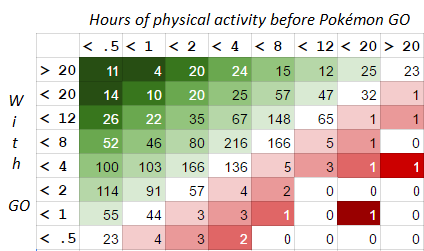
\includegraphics{Figures/change-in-physical-activity-table-colors}
	\caption{Change in physical activity with Pokémon GO}
	\label{fig:change-in-physical-activity}
\end{figure}

Respondents were also asked what activities lead to the increase in their physical activity, if they had become more physically active. Table \ref{tbl:physical-activity-sources} shows the number of respondents for each option out of 1823 respondents who reported an increase in physical activity.

\begin{table}[h]
	\centering
	\caption{Reasons for increased physical activity from Pokémon GO}
	\label{tbl:physical-activity-sources}
	\begin{tabular}{|c|c|c|c|}
		\hline
		\textbf{Detours} & \textbf{Errands} & \textbf{Pokéhunting} & \textbf{Other}\\\hline\hline
		1136 & 636 & 1576 & 89\\
		62\% & 35\% & 86\% & 5\%\\\hline
	\end{tabular}
\end{table}

It should be noted that 31 of these respondents (less than 2 \%) also chose the \emph{Not applicable} option, but it is uncertain what the implication of this is, given that they also selected other options. 25 of these 31 chose the same category for activity before and after, but because they are ranges it is still possible that they have increased activity within that range. The 6 remaining of those 31 reported more physical activity after Pokémon GO than before, so we can safely ignore the \emph{Not applicable} choice in their case. \todo{Should this be in Section \ref{sec:problems-with-survey} instead?}

The three categories \emph{Detours}, \emph{Errands} and \emph{Pokéhunting} were further explained in the question's options, see Appendix \ref{appendix:survey} \todo{(so I assume I don't have to repeat them here? Or should I?)}. Common examples of other activities leading to an increase in physical activity were players with dogs who walked them longer and more frequently to get in more play time or distance for their eggs, players who would walk during their breaks at work instead of sitting down, and players who went for longer or more frequent runs than previously. Many players who knew they should be going for walks but previously would not have, used Pokémon GO as a motivation to get outside and move around. Others found they enjoyed moving more and were motivated to start more rigorous exercise, while some even learned how to ride a bicycle so they could play more efficiently. \todo{Should I mention the respondents who said they increased physical activity for reasons unrelated to Pokémon GO? If so, here or in Section \ref{sec:problems-with-survey}?}

\todo{Mention 1) methods of transportation during play and 2) kilometers "walked" in the game? If so, here?}

\section{Analysis of Results for Change in Physical Activity}

The results were overwhelmingly positive. As seen in Table \ref{tbl:physical-activity-changed-category}, 73 \%, nearly three out of every four respondents, increased their physical activity enough to move up at least one category in physical activity after Pokémon GO compared to before. Table \ref{tbl:physical-activity-increased-multiple-categories} shows how many respondents from each initial category moved 2, 3, 4, 5 or 6 categories. Table \ref{tbl:physical-activity-average-categories-increased} shows how many categories players on average increased depending on their initial category. The \emph{Only increased} category shows the average increase for those who did in fact increase physical activity, while \emph{All} shows the numbers for all respondents who started within the respective category, including those who remained stable and those who decreased physical activity. \todo{Should these tables be moved to results?}

\begin{table}[h]
	\centering
	\caption{How many respondents increased physical activity by multiple categories?}
	\label{tbl:physical-activity-increased-multiple-categories}
	\begin{tabular}{|l|c|c|c|c|c|}
		\hline
		\textbf{Initial category} & \textbf{\( \geq2 \)} & \textbf{\( \geq3 \)} & \textbf{\( \geq4 \)}	& \textbf{\( \geq5 \)} & \textbf{\( \geq6 \)}\\
		\hline\hline
		30 minutes or less	& 317	& 203	& 103	& 51	& 25\\
							& 80\%	& 51\%	& 26\%	& 13\%	& 6\%\\\hline
		An hour or less		& 185	& 82	& 36	& 14	& 4\\
							& 57\%	& 25\%	& 11\%	& 4\%	& 1\%\\\hline
		2 hours or less		& 155	& 75	& 40	& 20	& n/a\\
							& 40\%	& 20\%	& 10\%	& 5\%	&\\\hline
		4 hours or less		& 116	& 49	& 24	& n/a	& n/a\\
							& 24\%	& 10\%	& 5\%	&		&\\\hline
		8 hours or less		& 72	& 15	& n/a	& n/a	& n/a\\
							& 18\%	& 4\%	& 		&		&\\\hline
		12 hours or less	& 12	& n/a	& n/a	& n/a	& n/a\\
							& 9\%	& 		&		&		&\\\hline
		\hline
		Total				& 857	& 424	& 203	& 85	& 29\\
							& 39\%	& 19\%	& 9\%	& 4\%	& 1\%\\\hline
	\end{tabular}
\end{table}

\begin{table}[h]
	\centering
	\caption{How many categories on average did players increase physical activity?}
	\label{tbl:physical-activity-average-categories-increased}
	\begin{tabular}{|l|c|c|}
		\hline
		\textbf{Initial category} & \textbf{Only increased} & \textbf{All}\\
		\hline\hline
		30 minutes or less	& 2.91	& 2.74\\
		An hour or less		& 2.16	& 1.83\\
		2 hours or less		& 1.90	& 1.57\\
		4 hours or less		& 1.57	& 1.06\\
		8 hours or less		& 1.40	& 0.75\\
		12 hours or less	& 1.20	& 0.45\\
		20 hours or less	& 1.00	& 0.23\\
		More than 20 hours	& n/a	& -0.27\\
		\hline
		Total				& 2.00	& 1.43\\\hline
	\end{tabular}
\end{table}

Because more than 92 \% of our respondents are adults by the WHO's definition of adults being aged 18-16, we are going to focus on the recommendations for adults. As discussed in Section \ref{sec:lit-study-physical-activity}, the WHO recommends that adults do at least 150 minutes of moderate-intensity physical activity per week. Using this recommendation, we categorize the players who are physically active less than this (the lower three categories) as \emph{Low activity} players. Respondents within the \emph{4 hours or less} and \emph{8 hours or less} categories will be categorized as \emph{Moderate activity} players, while the three remaining categories are \emph{High activity} players.

\begin{table}
	\centering
	\caption{Low/moderate/high activity players}
	\label{tbl:physical-activity-low-moderate-high}
	\begin{tabular}{|l|c|c|c|c|}
		\hline
		\textbf{Activity level}	& \textbf{Before}	& \textbf{After}	& \textbf{Change}	& \textbf{Categories increased}\\
		\hline\hline
		Low		& 1103	& 407	& -696	& 2.06\\
				& 50\%	& 19\%	& -63\%	&\\\hline
		Moderate& 871	& 1081	& 210	& 0.92\\
				& 40\%	& 49\%	& 24\%	&\\\hline
		High	& 219	& 705	& 486	& 0.31\\
				& 10\%	& 32\%	& 222\%	&\\\hline
	\end{tabular}
\end{table}

We see that while 50 \% of respondents were of low activity before Pokémon GO, this group only consisted of 19 \% of the respondents after Pokémon GO, a decrease of over 60 \%. The effect was larger for the lower activity ranges, where the number of respondents who had previously been active 30 minutes or less per week decreased by 92 \%, while the number who had previously been active between 1 and 2 hours per week only decreased by 30 \%. This is partly because the \emph{2 hours or less} category also saw an influx of players from the lower categories, but also because the lower ranges were narrower and thus easier to transcend. However, from Table \ref{tbl:physical-activity-average-categories-increased} we see that more than 50 \% of the respondents from the \emph{30 minutes or less} category increased their activity to a moderate level by jumping 3 or more categories, with the average number of categories increased for respondents initially placed in this category was 2.74.

The number of moderate activity players increased by 24 \%, which does not seem like a huge increase. However, paired with the fact that the number of high activity players more than tripled with a 222 \% increase, the number becomes more impressive, as this means the moderate activity category also "lost" quite a few of the players originally in this category. Respondents in the moderate activity category increased activity by a little less than one category on average. While this is not an enormous shift for these players, it places them safely within the range of the WHO's recommended weekly activity.

High activity players increased activity by 0.31 categories on average, with the majority of these increases coming from the players who had initially been active 12 hours or less. The initial members of the \emph{More than 20 hours} category decreased by 0.27 categories on average. The sample size was very small, however, consisting of only 26 respondents initially. The 0.27 category decrease is the result of three individuals and does not take into account that those in the \emph{More than 20 hours} category were unable to increase in category and that there were some respondents who mentioned in comments that they had in fact increased activity by 5-10 hours. It is however plausible that balancing a high physical activity week with playing Pokémon GO can be difficult, resulting in a slight decrease in physical activity from participating in game activities such as "camping" lures or nests. \todo{More on low-movement activities such as "camping".}

\todo{Althoff et al. ("Influence of Pokémon Go on Physical Activity ...") is highly relevant here and probably has some}

From Table \ref{tbl:physical-activity-sources}, we see that 62 \% of respondents listed \emph{Detours} as a cause for increased physical activity, while 86 \% listed \emph{Pokéhunting}. If and when a player stops playing Pokémon GO, they will no longer go out with the primary goal of catching or playing Pokémon. It is also unlikely that they will take detours when there is no goal with the detour other than taking it for the added activity. This unfortunately means that an increase in physical activity that originated from these sources is likely to revert should these players give up the game. 35 \% of respondents said they had started walking, biking \todo{(is "biking" too informal?)} or similar when performing errands or other day-to-day activities where they would previously have used some other mode of transportation such as a car. If these players stop playing the game, they could feasibly keep up this new routine, having realized it's not only possible to perform the activities without a car, but it also feels better to stay active, though it is unlikely to be the case for all of these players. For some members of the low activity category, being physically active more than before helped them realize they felt better with some physical activity in their routine, and some of these players started exercising outside of this. \todo{Check back on this paragraph later. Also needs to mention the follow-up results}

\todo{Only 19 \% left in low activity! Maybe in discussion/reflection/conclusion?}


\section{Results for Weight Loss, Feeling Healthier and Skipping Unhealthy Activities}

This section presents the results for the player survey questions related to Research Questions \ref{RQ2.4} and \ref{RQ2.5}. Table \ref{tbl:lost-weight-or-feeling-healthier} shows the categorized responses of 1478 respondents to the question \emph{Have you lost weight or in other ways feel more healthy than before you started playing Pokémon GO?}.

\begin{table}[h]
	\centering
	\caption{\emph{Have you lost weight or in other ways feel more healthy than before you started playing?} responses}
	\label{tbl:lost-weight-or-feeling-healthier}
	\begin{tabular}{|c|c|c|c|}
		\hline
		\textbf{Yes}	& \textbf{No}	& \textbf{N/A}	& \textbf{Unknown}\\
		\hline\hline
		738		& 671	& 19	& 50\\
		50\%	& 45\%	& 1\%	& 3\%\\\hline
	\end{tabular}
\end{table}

The \emph{No} respondents are players who did not experience any weight loss or improvement to health from playing the game. The \emph{Unknown} respondents did not know whether they had experienced any changes, and while some of them said \emph{"Probably"}, they have not been constrained to this category \todo{(is that necessary to mention?)}. The \emph{N/A} category are players who were already experiencing weight loss or changes to their health situation from other sources, such as diets, exercising or illnesses, prior to starting Pokémon GO. Their weight or health improvement progress continued while playing, but is assumed to be unrelated to Pokémon GO as the improvement had already started before they started playing, and these respondents were adamant that playing had not had an effect.

The \emph{Yes} category are the respondents who reported either weight loss or an improvement to one or more areas of their health. Out of these 738 respondents, 155 (21 \%) reported that they had lost weight. Other respondents reported a loss in body fat and/or gain in muscle mass while remaining at the same weight, while some noted a decrease in pant size while being unsure about changes to their weight. The most commonly reported improvement besides weight loss and generally feeling healthier was improved stamina or endurance, being able to walk or run faster, further and longer than before. Other improvements reported include eating and drinking better (drinking more water to stay hydrated and being less inclined to eat junk food), gain of motivation to exercise more, better sleep, less stress, easier breathing and feeling more alert. Some players reported that playing had helped them quit smoking, while a few lowered their blood pressure, experienced a positive effect on illnesses such as anemia, or an improved effect from their medication. Some players also used this question to note an improvement to mental health or happiness, which will be discussed further in Chapter \ref{chapter:player-study-mental}.

Players were also asked whether they had skipped any unhealthy activities in favor of playing Pokémon GO. Table \ref{tbl:skipping-unhealthy-activities} shows the 1629 responses to this question.

\begin{table}[h]
	\centering
	\caption{\emph{Have you skipped out on less healthy activities that you otherwise would have engaged in due to playing Pokémon Go instead?} responses}
	\label{tbl:skipping-unhealthy-activities}
	\begin{tabular}{|c|c|c|c|c|}
		\hline
		\textbf{Yes} & \textbf{No} & \textbf{Both} & \textbf{Opposite} & \textbf{N/A}\\
		\hline\hline
		415		& 1160	& 4		& 20	& 30\\
		25\%	& 71\%	& 0.25\%& 1\%	& 2\%\\\hline
	\end{tabular}
\end{table}

The \emph{No} category did not skip any activities they deemed unhealthy in favor of playing Pokémon GO, while the \emph{Yes} category did. The \emph{Both} category did less of one or more unhealthy activity, but more of another \todo{(too small to include? If so, which category to merge into, or just ignore?)}. The \emph{Opposite} category not only did not skip any unhealthy activities, but participated in more unhealthy activities because of the game than they would have without \todo{(merge into No-category and just mention these examples?)}. The \emph{N/A} category said they did not participate in any unhealthy activities neither before or after Pokémon GO.

\section{Analysis of Results for Weight Loss, Feeling Healthier and Skipping Unhealthy Activities}

While certainly not all individuals need to lose weight, the WHO reported that 39 \% of adults worldwide were overweight in 2014 \todo{[insert citation]}, while the NIDDK reported that more than 2 out of every 3 adults in the United States were overweight \todo{[insert citation]}. Therefore we can assume that the fact that over 10 \% of respondents lost weight is a positive thing overall. Out of the 84 subjects who responded with the amount of weight they had lost, the average respondent had lost just over 5.2 kg, ranging from 0.5 to 18.5 kg. However, not knowing the initial weight of these respondents, it is difficult to determine exactly how positive this is, as discussed in \ref{sec:problems-with-survey}.

There are a few other points to note regarding the weight loss data. Some players categorized as \emph{Yes}-respondents started diets or more focused exercise after they started playing Pokémon GO, meaning it is difficult to determine the impact of playing Pokémon GO in their weight loss. However, for many or most of these respondents, the lifestyle change was inspired by the increased activity and health improvements already experienced from playing Pokémon GO.

Others who lost weight were already underweight and actually needed to gain weight. While their loss of weight was not positive, most of these players also experienced a positive effect such as improvements to mental health, or help with physical conditions such as anemia.

Some of the \emph{No} players not only did not experience an improvement, but worsened their current state by exercising less or adopting bad habits such as eating more junk food or going to bars drinking when they otherwise would not have done so. These are mostly the same players as represented by the \emph{Opposite} category in Table \ref{tbl:skipping-unhealthy-activities}, although there are some players that do not overlap.

As seen in Table \ref{tbl:skipping-unhealthy-activities}, 25 \% of respondents said that they skipped unhealthy activities in favor of playing Pokémon GO. While the activities in question for a lot of these players (roughly 38 \%) were primarily watching TV or playing video games at home, it's not unlikely that many of these activities would have included snacks that were not consumed while out playing. There were also quite a few (more than 26 \%) who went out to play Pokémon instead of going to bars or otherwise consume alcohol. Others cut down on junk food, and some stopped snacking and overeating in general. Some players even managed to stop smoking due to playing. There were unfortunately also some players who started drinking more because their local bars had good access to Pokéstops, so sitting at those bars with lures became a habit. \todo{Is this paragraph ok as is?}

There is nothing about Pokémon GO itself that causes the physical health benefits experienced by its players, which are all due to the lifestyle changes playing the game brought, primarily the increased physical activity. However, it managed to motivate many players to experience this increased physical activity without marketing as an exercise application, and 50 \% of respondents experienced a tangible effect on their physical health from doing what they thought of as simply playing a game. \todo{Perhaps move this paragraph to reflection on results?}


\section{Results for Neglect and Negative Behavior}

The players who started exercising less or drinking more are not the only negative side effects of playing Pokémon GO. This section presents the results for the player survey questions related to Research Question \ref{RQ2.6}. Players were asked whether they had neglected other important areas of their life due to playing Pokémon GO, and 220 players responded that they had neglected to eat, drink or sleep enough. Some of these players became dehydrated, while others had little energy because of the lack of sleep. Three respondents neglected giving their feet the rest they needed and experienced serious problems because of this, where two developed tendinitis and one made a chronic condition worse. Some players were not used to spending large amounts of time outside during summer and experienced sunburns of varying severity.

Players were also asked whether they had trespassed, put themselves or others in dangerous situations or gotten into accidents. Almost 15 \% of the respondents had trespassed at least once, with 47 \% of them doing so knowingly. While trespassing often is uneventful and without significant risk, it has the potential to be dangerous in addition to being inconsiderate. 238 players, a little less than 11 \% of all the respondents, said they had put either themselves or others in one or more dangerous situations, with 94 \% endangering themselves and 33 \% admitting to endangering others. 92 players had been in accidents because of the game, whereof 2 were accidents with serious injury or property damage.

Of the players who had either endangered themselves or others, or gotten into accidents, 231 respondents chose to elaborate on the events. Table \ref{tbl:danger-or-accidents-elaboration} shows the most common causes for accidents and sources of endangerment.

\begin{table}[h]
	\centering
	\caption{\emph{If you have put yourself or others in dangerous situations, or gotten into accidents, because of Pokémon Go, could you elaborate?} categorized responses}
	\label{tbl:danger-or-accidents-elaboration}
	\begin{tabular}{|c|c|c|c|c|c|}
		\hline
		Driving	& Surroundings	& Traffic	& Bicycle	& Alone at night	& Bad neighborhood\\
		\hline\hline
		90		& 38			& 36		& 28		& 15				& 8\\
		39\%	& 16\%			& 16\%		& 12\%		& 6\%				& 3\%\\\hline
		%		\textbf{Category} & \textbf{Endangered} & \textbf{Accident} & \textbf{Total}\\
		%		\hline\hline
		%		Car				& 84	& 7		& 90\\
		%						& 36\%	& 3\%	& 39\%\\\hline
		%		Surroundings	& 22	& 26	& 38\\
		%						& 9\%	& 11\%	& 16\%\\\hline
		%		Traffic			& 33	& 10	& 36\\
		%						& 14\%	& 4\%	& 16\%\\\hline
		%		Bicycle			& 17	& 16	& 28\\
		%						& 7\%	& 7\%	& 12\%\\\hline
		%		Alone at night	& 11	& 1	& 28\\
		%						& 7\%	& 7\%	& 12\%\\\hline
	\end{tabular}
\end{table}

The \emph{Driving} category respondents put themselves or others in danger by playing Pokémon GO while driving, or were in accidents with their car because they were playing Pokémon GO.

The \emph{Surroundings} category are respondents who were not paying attention to their surroundings while playing (mostly on foot), many of whom got into accidents because of it.

The \emph{Traffic} category are respondents who either did not pay sufficient attention when walking in or around traffic because they were playing Pokémon GO, or drivers who got into or narrowly avoided accidents because someone else was playing.

The \emph{Bicycle} category are players who were playing while riding a bicycle, exposing themselves to risk and/or getting into accidents because of it. Another 5 respondents reported similar experiences using other methods of transportation, such as skateboards or \emph{hovedboards} \todo{(include picture of a hoverboard?)}.

The \emph{Alone at night} category are respondents who put themselves at risk by walking outside alone at night when they usually would not have, while the \emph{Bad neighborhood} category are players who ventured into dangerous neighborhoods to play.

\section{Analysis of Results for Neglect and Negative Behavior}

Just as any other engaging activity, Pokémon GO caused some players (roughly 10 \% of the total respondents) to neglect sleep, eating enough or staying hydrated. While this is not a new phenomenon, the extra physical activity Pokémon GO players are exposed to compared to activities such as computer games means that staying hydrated is extra important, particularly in the summer heat. On the game's loading screen, it encourages players to be aware of their surroundings. This place could also be used to remind players to stay hydrated while playing and encourage players to drink enough water. Another possible option is making every few Pokéstops claimed give this same reminder and encouragement, possibly based on geographic location or the current season to avoid making players tired of these warnings when the weather is less warm and prone to cause dehydration.

The greater issue, however, are players who drive and play at the same time. It is widely known \todo{[cite WHO]} that using a mobile phone while driving greatly increases chances of accidents happening, yet many still do it. That almost 2 out of every 5 respondents who endangered themselves or others were doing so by playing while driving is a serious issue that Niantic did make an effort to fix by blocking the game with a warning whenever the player was detected to be moving too fast to be on foot, asking the player not to play while driving, as seen in Figure \ref{fig:do-not-play-and-drive}. Some of these players did not even seem to realize that they were endangering not only themselves, but also other innocent people with their actions, as shown by the difference in number of respondents who said they were playing while driving and the number who said they had put themselves or others in danger. Only 7 of these players (less than 8 \% of the drivers) were involved in accidents because of playing while driving, and all of them were minor accidents with slight damage to the car, but if any of these 90 players had been less lucky, their actions could have been fatal. \todo{(include picture of in-game warning here)}}

\begin{figure}[h]
	\centering
	\caption{\emph{Do not play Pokémon GO while driving} in-game warning}
	\label{fig:do-not-play-and-drive}
\end{figure}

Bikers were not quite as lucky while playing, and 16 out of the 28 (or 57 \%) got into accidents where they either hurt themselves, their bike, or hit someone else. Most of these accidents were minor, but one player hit an unexpectedly high speed bump while not paying attention and ended up with a broken arm. These numbers, while a small sample size, indicate that playing Pokémon GO while biking is not a good combination. While a total of 575 players reported using a bicycle as a method of transportation while playing, it is unknown how many of these played actively while on the bike, and we will have to rely on the numbers for those who explicitly mentioned playing while biking. It is however possible that the portion of players who play while riding a bicycle is larger, as several retailers reported increased sales of phone holders for bicycles. This would imply that playing while biking is relatively safer than originally assumed, but players should still show caution.

As previously mentioned and seen in Figure \ref{fig:loading-screen-aware-of-surroundings}, the loading screen for the game encourages players to remain aware of their surroundings while playing, and with good reason. Of the players who did not pay attention to their surroundings around traffic, 10 (28 \%) were involved in accidents. These players wandered into the street without looking properly or walked too close to the edge of the sidewalk and got hit by cyclists or side mirrors of cars. That only ten of these players were involved in accidents, and that none of them had serious consequences, is likely thanks to a good dose of luck \todo{(too informal?)}, and similarly to those who play and drive, this could have gone much worse with less luck.

26 (68 \%) of the players who did not pay attention to their surroundings in general were involved in accidents. While this portion seems staggeringly high, based on general observation of players in the wild, a much larger percentage of players than the 38 who mentioned it were playing without paying particularly close attention to their surroundings. It is likely that the 38 players who mentioned it were the ones who were involved in accidents or near-accidents because of it, while the majority of the other players avoided this. The players in this category who were involved in accidents experienced events such as crashing into things (signs, lamp posts, parked cars, low balconies and similar), kicking things or misplacing their step. There were sprains, bruises and minor cuts, but no serious accidents.

\begin{figure}[h]
	\centering
	\caption{Game loading screen encouraging players to remain aware of their surroundings while playing}
	\label{fig:loading-screen-aware-of-surroundings}
\end{figure}

The players in the \emph{Alone at night} and \emph{Bad neighborhood} categories ventured out into the night to play Pokémon when or where they should not have, and without Pokémon would not either. For the most part, no harm came to them, with the exception of two players: one player was mugged \todo{[insert link to newspaper article about it?]} and another was shot after, but not hit. Still, the placement of Pokéstops and spawns can cause players to take unnecessary risks and venture into areas they should not be in. This is also the reason why some areas, such as airports, often have no spawns or Pokéstops. Another similar cause, if a little more innocent, is players who followed paths on the map that were not actually paths in reality, ending up in minor accidents such as those experienced by the players who were unaware of their surroundings.

The other serious accident respondents were involved in because of playing Pokémon GO was a player who experienced serious damage to his car because he had driven out to play Pokémon. He was not playing while driving, but had he not gone out to play, the damage would not have happened. Other players reported similar, if less severe events with flat tires and minor damages to their cars because they had brought their car out to play.


% Chapter
\chapter{Mental Health Effects}
\label{chapter:player-study-mental}
\lhead{Chapter \ref{chapter:player-study-mental}. \emph{Player Study - Mental Health Effects}}

This chapter examines the survey results in the context of determining th game's effect on the mental health of its players. The questions in Table \ref{tbl:rg3-survey-questions} and their answers are the main focus of this chapter, but relevant answers to other questions are also included.

\section{Results for Change in Social Activity}

This section presents the results for the player survey questions related to Research Questions \ref{RQ3.1} and \ref{RQ3.2}. A total of 2192 subjects responded to the questions \emph{"In an average week, during your spare time, how much time did you spend socializing with other people (in person, outside your home) before you started playing Pokémon Go?"} and \emph{"In an average week, during your spare time, how much time do you spend socializing with other people (in person, outside your home) since you started playing Pokémon Go?"}. Table \ref{tbl:social-activity-before-and-after} shows the number of responses to each question (column 2 and 3 respectively), as well as the change \todo{(should it say delta?)}, within each time category. Percentages for the \emph{Before} and \emph{After} columns are the percentage of total respondents for the respective category, while the percentage in the \emph{Change} column shows the relative increase or decrease (negative percentages) for that category. Note that the percentages are rounded to the closest integer, and due to rounding errors, the percentages in column 2 and 3 both sum to 99 \% \todo{(consider removing this and similar remarks and just mention it in problems with survey section)}. \todo{This paragraph is more or less a carbon copy of the corresponding section in physical health chapter. Is that ok?}

\begin{table}[h]
	\centering
	\caption{Social activity before and after Pokémon GO}
	\label{tbl:social-activity-before-and-after}
	\begin{tabular}{|l|c|c|c|}
		\hline
		\textbf{Hours of activity} & \textbf{Before} & \textbf{After} & \textbf{Change} \\\hline\hline
		30 minutes or less	& 245 & 138 & -107\\
		& 11\% & 6\% & -44\%\\\hline
		An hour or less & 220 & 155 & -65\\
		& 10\% & 7\% & -30\%\\\hline
		2 hours or less & 396 & 314 & -82\\
		& 18\% & 14\% & -21\%\\\hline
		4 hours or less & 499 & 492 & -7\\
		& 23\% & 22\% & -1\%\\\hline
		8 hours or less & 416 & 478 & 62\\
		& 19\% & 22\% & 15\%\\\hline
		12 hours or less	& 204 & 307 & 103\\
		& 9\% & 14\% & 50\%\\\hline
		20 hours or less	& 116 & 175 & 59\\
		& 5\% & 8\% & 51\%\\\hline
		More than 20 hours	& 96 & 133 & 37\\
		& 4\% & 6\% & 39\%\\\hline
	\end{tabular}
\end{table}

Where Table \ref{tbl:social-activity-before-and-after} shows how many respondents shows the changes within each time range of social activity, Table \ref{tbl:social-activity-change-or-stable} shows the number of respondents who became less socially active, more socially active or did not change their amount of social interaction.

\begin{table}[h]
	\centering
	\caption{How many respondents changed social activity time categories?}
	\label{tbl:social-activity-change-or-stable}
	\begin{tabular}{|c|c|c|}
		\hline
		\textbf{Decreased} & \textbf{Stable} & \textbf{Increased}\\\hline\hline
		74		& 1353		& 765\\
		3\%		& 62\%		& 35\%\\\hline
	\end{tabular}
\end{table}

\section{Analysis of Results for Change in Social Activity}

\section{Social Interaction}
\label{sub:mental-health-social}

\todo{Mention division of tasks (searching for nearby pokes, scoping out gyms, and transporter/player), and that players on different teams still can cooperate and be on good terms}

\section{Exercise}

\section{A Sense of Purpose}

\section{Disappointment}

\section{Negative Behavior and Adversarial Relationships}

\part{Discussion and Conclusion}
\label{part:discussion-and-conclusion}
% Chapter 6 - Discussion

\chapter{Discussion}

% Section 1 - General reflection on results
\section{Reflection on results}

\todo{This section should reflect on the results, and explain any choices or mistakes in the process that may have negatively affected the collection of results. Could also include personal speculation on the answers.}

% Section 2 - Reactions from non-players
\section{Reaction From Non-Players}

\todo{This section should discuss reactions from non-players (general attitudes in the community) and perhaps media.}

% Section 2 - The future of Pokémon Go and similar games
\section{Future of Pokémon Go and Similar Games}

\todo{This section speculates on the future of Pokémon Go and similar games, with basis in observations and the results from the survey.}
% Chapter 7 - Conclusion

\chapter{Future Work}
\todo{Future work in the research, e.g. sample other groups, more on financial impact etc}

\chapter{Conclusion}
\todo{This chapter should contain the conclusion, which is a summary of the findings and what has been written in the paper.}

%----------------------------------------------------------------------------------------
%  THESIS CONTENT - APPENDICES
%----------------------------------------------------------------------------------------

\addtocontents{toc}{\vspace{2em}} % Add a gap in the Contents, for aesthetics

\appendix % Cue to tell LaTeX that the following 'chapters' are Appendices

% Include the appendices of the thesis as separate files from the Appendices folder
% Uncomment the lines as you write the Appendices

% Appendix: Survey questions
\chapter{Player Survey - Final, English version}
\label{appendix:survey}

\chapter{Follow-up Survey}
\label{appendix:follow-up}
%\input{Appendices/AppendixB}
%\input{Appendices/AppendixC}

\addtocontents{toc}{\vspace{2em}} % Add a gap in the Contents, for aesthetics

\backmatter

%----------------------------------------------------------------------------------------
%  BIBLIOGRAPHY
%----------------------------------------------------------------------------------------

\label{Bibliography}

\lhead{\emph{Bibliography}} % Change the page header to say "Bibliography"

\bibliographystyle{apalike} % Use the "unsrtnat" BibTeX style for formatting the Bibliography
\bibliography{Bibliography} % The references (bibliography) information are stored in the file named "Bibliography.bib"

\end{document}  